% ---------------------------------------------------------------
% Preamble
% ---------------------------------------------------------------
%\documentclass[a4paper,fleqn,longmktitle]{cas-sc}
\documentclass[a4paper,fleqn]{cas-dc}
%\documentclass[a4paper]{cas-dc}
%\documentclass[a4paper]{cas-sc}
% ---------------------------------------------------------------
% Make margins bigger to fit annotations. Use 1, 2 and 3. TO be removed later
%\paperwidth=\dimexpr \paperwidth + 6cm\relax
%\oddsidemargin=\dimexpr\oddsidemargin + 3cm\relax
%\evensidemargin=\dimexpr\evensidemargin + 3cm\relax
%\marginparwidth=\dimexpr \marginparwidth + 3cm\relax
% -------------------------------------------------------------------- 
% Packages
% --------------------------------------------------------------------
% Figure packages
\usepackage{graphicx,float}
\restylefloat{table}
\usepackage{adjustbox}
% Text, input, formatting, and language-related packages
\usepackage[T1]{fontenc}
\usepackage{subcaption}

\usepackage{nomencl}
\makenomenclature

\usepackage{etoolbox}
\renewcommand\nomgroup[1]{%
	\item[\bfseries
	\ifstrequal{#1}{A}{Latin symbols}{%
		\ifstrequal{#1}{B}{Non-lation symbols}{%
			\ifstrequal{#1}{C}{Greek symbols}{%
				\ifstrequal{#1}{D}{Abberivations}{
	}}}}%
	]}
\newcommand{\nomunit}[1]{%
	\renewcommand{\nomentryend}{\hspace*{\fill}#1}}


% TODO package
\usepackage[bordercolor=gray!20,backgroundcolor=blue!10,linecolor=black,textsize=footnotesize,textwidth=1in]{todonotes}
\setlength{\marginparwidth}{1in}
% \usepackage[utf8]{inputenc}
% \usepackage[nomath]{lmodern}

% Margin and formatting specifications
%\usepackage[authoryear]{natbib}
\usepackage[sort]{natbib}
\setcitestyle{square,numbers}

 %\bibliographystyle{cas-model2-names}

\usepackage{setspace}
\usepackage{subfiles} % Best loaded last in the preamble

% \usepackage[authoryear,longnamesfirst]{natbib}

% Math packages
\usepackage{amsmath, amsthm, amssymb, amsfonts, bm, nccmath, mathdots, mathtools, bigints, ulem}

\usepackage{tikz}
\usepackage{pgfplots}
\usetikzlibrary{shapes.geometric,angles,quotes,calc}

\usepackage{placeins}

\usepackage[final]{pdfpages}

\usepackage{multirow}

\usepackage[switch]{lineno}

% --------------------------------------------------------------------
% Packages Configurations
\usepackage{enumitem}
% --------------------------------------------------------------------
% (General) General configurations and fixes
\AtBeginDocument{\setlength{\FullWidth}{\textwidth}}	% Solves els-cas caption positioning issue
\setlength{\parindent}{20pt}
%\doublespacing
% --------------------------------------------------------------------
% Other Definitions
% --------------------------------------------------------------------
\graphicspath{{Figures/}}
% --------------------------------------------------------------------
% Environments
% --------------------------------------------------------------------
% ...

% --------------------------------------------------------------------
% Commands
% --------------------------------------------------------------------

% ==============================================================
% ========================== DOCUMENT ==========================
% ==============================================================
\begin{document} 
%  --------------------------------------------------------------------

% ===================================================
% METADATA
% ===================================================
\title[mode=title]{Global sensitivity analysis of a supercritical extraction model}
\shorttitle{GSA}

\shortauthors{OS}

\author[1]{Oliwer Sliczniuk}[orcid=0000-0003-2593-5956]
\ead{oliwer.sliczniuk@aalto.fi}
\cormark[1]
\credit{a}

%\author[1]{Pekka Oinas}[orcid=0000-0002-0183-5558]
%\credit{b}

%\author[1]{Francesco Corona}[orcid=0000-0002-3615-1359]
%\credit{c}

\address[1]{Aalto University, School of Chemical Engineering, Espoo, 02150, Finland}
%\address[2]{2}

\cortext[cor1]{Corresponding author}

% ===================================================
% ABSTRACT
% ===================================================
\begin{abstract}
	This study investigates the process of chamomile oil extraction from flowers. A parameter-distributed model consisting of a set of partial differential equations is used to describe the governing mass transfer phenomena in a cylindrical packed bed with solid chamomile particles under supercritical conditions using carbon dioxide as a solvent. The concept of quasi-one-dimensional flow is applied to reduce the number of spatial dimensions. The flow is assumed to be uniform across any cross-section, although the area available for the fluid phase can vary along the extractor. The physical properties of the solvent are estimated from the Peng-Robinson equation of state. The empirical correlations used in the model are based on laboratory experiments performed under multiple constant operating conditions: $30 - 40~^\circ$C, $100 - 200$ bar and $3.33-6.67 \cdot 10^{-5}$ kg/s. The first and higher-order Sobol indices were computed to assess separate and joined contribution of the operating conditions to the model output and its variance.
	
\end{abstract}

\begin{keywords}
	Supercritical extraction \sep Optimal design of experiments \sep Mathematical modelling
\end{keywords}

% ===================================================
% TITLE
% ===================================================
\maketitle

% ===================================================
% Section: Introduction
% ===================================================

\section{Introduction}
\linenumbers
%\subfile{Sections/introduction_imp}
Supercritical CO2 extraction is a green extraction method that uses carbon dioxide in a supercritical state (above its critical point of 31.1 $^\circ$C and 73.8 bar) to extract compounds from materials. This is one of the most popular applications of supercritical fluids, which was described by many researchers, for example \citet{Sodeifian2017}, \citet{Reverchon1993} and \citet{Sovova1994}. Traditional methods, such as distillation and organic solvent extraction, are commonly employed although they have drawbacks. Distillation involves high temperatures that can lead to the thermal degradation of heat-sensitive compounds. This limitation has increased the popularity of alternative techniques, such as supercritical fluid extraction. Supercritical CO$_2$ is attractive due to its distinctive properties: it is inflammable, non-toxic and non-corrosive. Supercritical fluids can exhibit both gas- and liquid-like properties, allowing for adjustable dissolving power through changes in operating conditions.

Applications for supercritical carbon dioxide are not limited to extraction processes; they can also be used for impregnation, as described by \citet{Weidner2018} and \citet{Machado2022}. Impregnation is defined as modification of the properties of bulk substances by physically or chemically binding/adsorbing impregnates to a bulk material or surface, for example, the surface hydrophobisation. The main advantage of using supercritical CO$_2$ is that, after depressurisation, it desorbs from the surface and evaporates, leaving a solvent-free product. However, the main disadvantage of using carbon dioxide for impregnation is the low solubility of many drugs surface hydrophobisation. 
The study of \citet{Ameri2020} investigates the loading of lansoprazole into polymers using supercritical carbon dioxide and examines how various parameters, such as temperature, pressure and time, affect the drug loading efficiency. The results indicate that increasing any of these parameters enhances drug loading, with temperature having the most significant impact. \citet{Fathi2022} explored the use of supercritical carbon dioxide to enhance the bioavailability of ketoconazole by impregnation into water-soluble polymers, specifically polyvinylpyrrolidone and hydroxypropyl methylcellulose. Utilising a Box-Behnken design, the researchers optimised the impregnation process by varying pressure, temperature and time, achieving an increased drug loading range.

Another application of supercritical CO$_2$ is nanoparticle formation, as investigated by \citet{Padrela2018}, \citet{Franco2021} and \citet{Sodeifian2022}. Supercritical $CO_2$-assisted technologies enable the production of different morphologies of different sizes, including nanoparticles and nanocrystals, by modulating the operating conditions. Supercritical fluid-based processes have advantages over techniques conventionally employed to produce nano-sized particles or crystals, such as reduced use of toxic solvents. Moreover, the CO$_2$ can be removed from the final product by simple depressurisation. 
\citet{Sodeifian2018} investigated the solubility of Letrozole, a poorly water-soluble anticancer drug, in supercritical carbon dioxide with and without menthol as a solid co-solvent. The addition of menthol increased the solubility of Letrozole by 7.1 times compared to supercritical CO$_2$ alone. Using the rapid expansion of supercritical solutions with the solid co-solvent method, the average particle size of Letrozole was reduced to the nanoscale. Temperature was found to have the most significant impact on nanoparticle size reduction, while pressure had the least effect. 
The study of \citet{SaadatiArdestani2020} explored the preparation of phthalocyanine green nano pigment using supercritical carbon dioxide as an anti-solvent. The researchers employed the gas anti-solvent technique to achieve nano-sized pigment particles.
\citet{Sodeifian2019} analysed the production of amiodarone hydrochloride nanoparticles using ultrasonic-assisted rapid expansion of the supercritical solution in a liquid solvent method. The researchers achieved significant particle size reduction by optimising parameters such as pressure, temperature and polymeric stabiliser concentration. Characterisation techniques confirmed the successful formation of nanoparticles with improved properties.

Although the processes discussed are based on different phenomena, the outcome of these technologies strongly depends on the solubility in supercritical CO$_2$. The solubility of the solid in the solvent can be important for determining the partition coefficient for a potential impregnation and whether a cosolvent should be used in a supercritical extraction of a compound. Moreover, a good solute solubility not only accelerates the initial stages of the extraction but also reduces the time of the extraction process. Multiple researchers, such as \citet{Bagheri2025}, \citet{Tabebordbar2024}, \citet{SheikhiKouhsar2024} or \citet{Bagheri2022}, have conducted extensive research to measure the solubility of different solutes in the supercritical CO$_2$ and on the development of mathematical models. Several methods, including density-based correlations and equation of state, are used for correlations of solute solubility in the supercritical CO$_2$. The semi-empirical models are often used due to their ease of use and the absence of the need for physicochemical properties like sublimation pressure and critical features, which cannot be directly measured experimentally.

The present study investigates the extraction of essential oil from chamomile flowers (\textit{Matricaria chamomilla L.}) via supercritical fluid extraction techniques in addition to the modelling of this process. Chamomile is a medicinal herb widely cultivated in southern and eastern Europe - in countries such as Germany, Hungary, France and Russia. It can also be found outside Europe, for instance in Brazil, as discussed by \citet{Singh2011}. Chamomile is distinguished by its hollow, bright gold cones that house disc or tubular florets surrounded by about fifteen white ray or ligulate florets. The plant has been utilised for its medicinal benefits, serving as an anti-inflammatory, antioxidant, mild astringent, and healing remedy. Chamomile extracts are widely used to calm nerves and mitigate anxiety, hysteria, nightmares, insomnia and other sleep-related conditions, according to \citet{Srivastava2009}. \citet{Orav2010} reported that oil yields from dried chamomile samples ranged from 0.7 to 6.7 mL/kg. The highest yields of essential oil, between 6.1 mL/kg and 6.7 mL/kg, were derived from chamomile sourced from Latvia and Ukraine. In comparison, chamomile from Armenia exhibited a lower oil content of 0.7 mL/kg. \citet{Milovanovic2023} extracted oils from Roman chamomile seeds in a two-stage process. First, supercritical carbon dioxide at pressures of up to 450 bar and temperatures up to 60 $^\circ$C was used for the first extraction. Then, the oil was re-extracted using supercritical CO$_2$ with the addition of ethanol. Through optimisation of the operating pressure, temperature, production cost, fraction of milled seeds and addition of co-solvent, the amount of separated chamomile oil increased from 2.4 to 18.6\% and the content of unsaturated fatty acids up to 88.7\%.

The literature offers various mathematical models to describe the extraction of valuable compounds from biomass. Selecting a process model is case-dependent and requires analysis of each model's specific assumptions about mass transfer and thermodynamic equilibrium. Depending on the case, two approaches can be considered when developing a mathematical model for the extraction process. A model based on multiple regression can be used if the relation between inputs and outputs is the only one of interest. \citet{Sodeifian2017a} investigated the influence of pressure, temperature and particle size on the extraction efficiency of oil from \textit{Dracocephalum kotschyi Boiss} seed. A second-order polynomial model was applied to obtain the corresponding response surface and to identify the optimum operating conditions. The study of \citet{Sodeifian2017b} investigates the extraction of essential oil from Eryngium billardieri, focusing on optimising the extraction conditions and developing a mathematical model based on the second-order polynomial to predict the process yield. The researchers employed a simulated annealing algorithm to optimise parameters such as pressure, temperature and extraction time, aiming to maximise oil extraction efficiency.

Alternatively, a first-principle model can be derived and applied to cover not only the input-output relations, but also the phenomena occurring in the system. This approach allows for a more detailed representation of the system behaviour, but requires deeper understanding of the underlying physics and more rigorous experiments. \citet{Sliczniuk2025a} provides a list of studies on SFE, including modelling approaches, raw materials, and operating conditions. Below some of the most popular SFE models are discussed.

\citet{Goto1996} presented the shrinking core (SC) model, which describes a process of irreversible desorption followed by diffusion through the pores of a porous solid. When the mass transfer rate of the solute in the non-extracted inner region is significantly slower than in the outer region, where most of the solute has already been extracted or when the solute concentration exceeds its solubility in the solvent, a distinct boundary may form between the inner and outer regions. As extraction progresses, the core of the inner region shrinks. The model envisions supercritical CO$_2$ extraction as a sharp, inward-moving front, with a completely non-extracted core ahead of the front and a fully extracted shell behind it.

\citet{Sovova1994} proposed the broken-and-intact cell (BIC) model, which assumes that a portion of the solute, initially stored within plant structures and protected by cell walls, is released during the mechanical breakdown of the material. The solute located in the region of broken cells near the particle surface is directly exposed to the solvent, while the core of the particle contains intact cells with undamaged walls. This model describes three extraction phases: a fast extraction phase for accessible oil, a transient phase and a slow phase controlled by diffusion. The model has been successfully applied to the extraction of grape oil (\citet{Sovova1994b}) and caraway oil (\citet{Sovova1994a}).

The supercritical fluid extraction (SFE) process can be treated similarly to heat transfer, considering solid particles as spheres cooling down in a uniform environment. \citet{Bartle1990} introduced the hot ball diffusion (HBD) model, where spherical particles with a uniformly distributed solute diffuse similarly to heat diffusion. Unlike the BIC model, where the solute is readily available on the particle surface, the HBD model is suitable for systems with small quantities of extractable materials and is not limited by solubility. The model is particularly relevant when mass transfer is controlled by internal diffusion, allowing results from single particles to be extended to the entire bed under uniform conditions. \citet{Reverchon1993} have further elaborated on the HBD model and used it to simulate extraction processes.

\citet{Reverchon1996} proposed a model for the extraction of essential oils that are mainly located inside vegetable cells in organelles called vacuoles. Only a small fraction of essential oil might be near the particle surface due to the breaking up of cells during grinding or in epidermal hairs located on the leaf surface. The fraction of oil freely available on the particle surface should not be significant in the case of SFE from leaves. Consequently, SFE of essential oil from leaves should be controlled mainly by internal mass-transfer resistance. Therefore, the external mass-transfer coefficient was neglected in the development of Reverchon's model (\citet{Reverchon1996}). The mass balances were developed with the additional hypotheses that axial dispersion can be neglected and that the solvent density and flow rate are constant along the bed.

This work builds upon the linear kinetic model suggested by \citet{Reverchon1996}, deriving fundamental governing equations to develop a comprehensive model for the chamomile oil extraction process. The model aims at control-oriented simplicity, assuming semi-continuous operation within a cylindrical vessel. The process involves a supercritical solvent being pumped through a fixed bed of finely chopped biomass to extract the solute, followed by separation of the solvent and solute in a flush drum to collect the extract. Parameters such as pressure ($P$), feed flow rate ($F$) and inlet temperature ($T_{in}$) are adjustable and measurable, while the outlet temperature ($T_{out}$) and the amount of product at the outlet can only be monitored. Figure \ref{fig: SFE_drawing} presents a simplified process flow diagram.

\begin{figure}[h!]
	\centering
	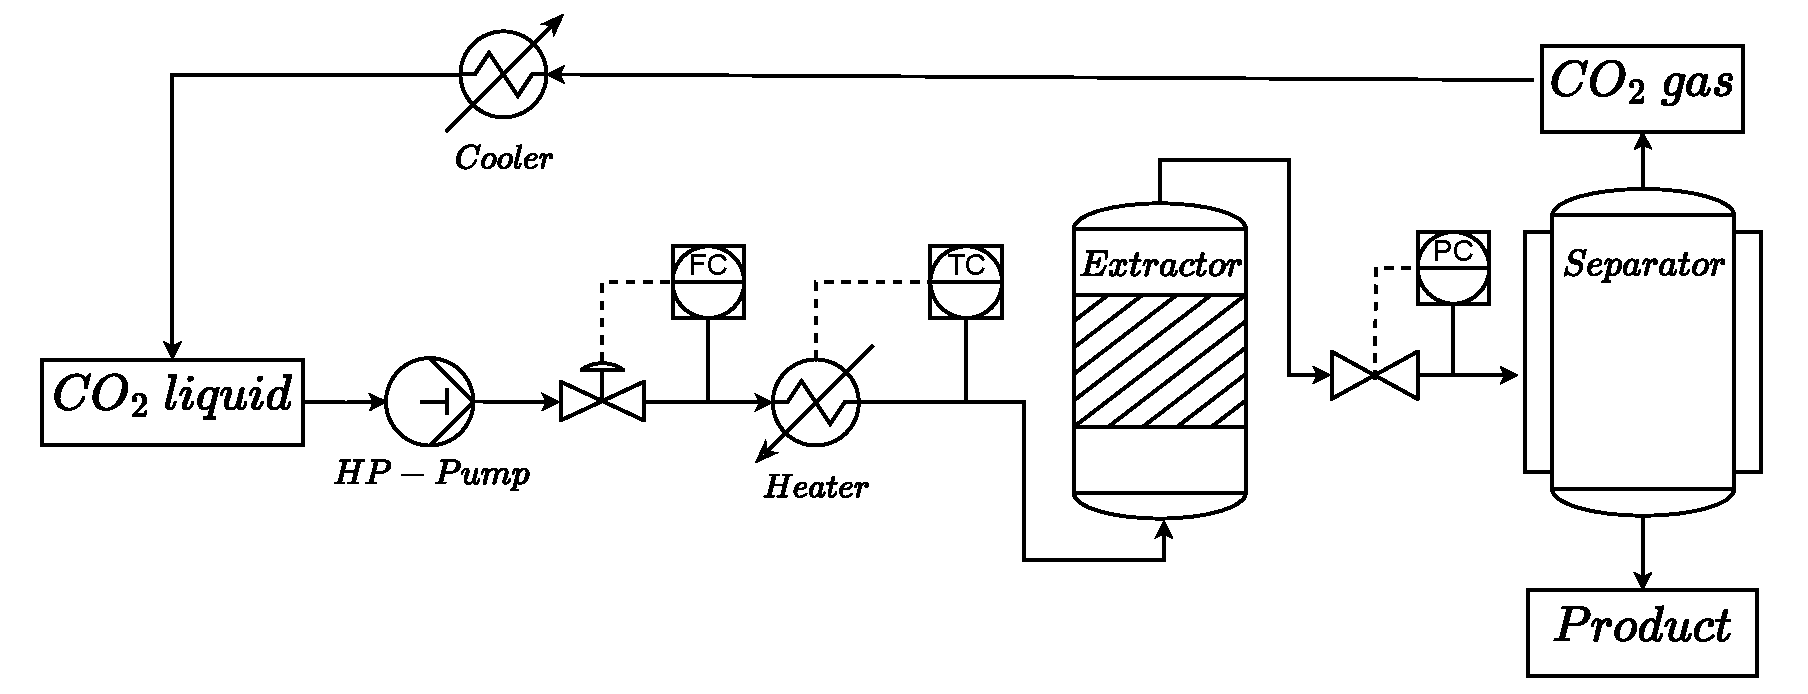
\includegraphics[width=\columnwidth]{Figures/PFD.drawio.pdf}
	\caption{Process flow diagram.}
	\label{fig: SFE_drawing}
\end{figure}

%\subfile{Sections/Literature_Review}

One limitation of the model development process is the need to capture the required physical behaviour while maintaining interpretability. However, models inherently contain a large number of parameters, creating a complex network of dependencies. Model analysis techniques and sensitivity analysis provide theoretical frameworks to identify dependencies between model output and its parameters. As discussed by many authors such as \citet{Jamett2015}, \citet{Duong2016} or \citet{Lucay2015}, sensitivity analysis (SA) is the study of uncertainties in the responses (outputs) of a mathematical model, which can be attributed to different sources of uncertainty in the values of the model parameters (input variables). These uncertainties can be epistemic (related to lack of knowledge) or stochastic (due to randomness). The effects of these uncertainties must be examined to avoid poor design, safety issues, and unreliable systems, among other problems. SA methods can help to analyse the effect of uncertainties. However, they can be computationally expensive for complex issues of chemical processes.

As noted by \citet{Gan2014}, the literature presents several methods for performing SA. In general, these methods can be classified into two main groups: local SA and global SA (GSA). The local SA explores changes in the model response by varying one parameter while keeping other parameters constant. In contrast, the GSA examines changes in the model response by simultaneously varying all parameters.

% ===================================================
% Section: Main
% ===================================================

%\subfile{Sections/Model}
\section{Materials and methods} \label{CH: Materials and methods}

\subsection{Governing equations} \label{CH:Governing_equations_chapter}
The governing equations for a quasi-one-dimensional flow were derived by following the work of \citet{Anderson1995}. A quasi-one-dimensional flow refers to a fluid flow scenario which assumes that the flow properties are uniformly distributed across any cross-section. This simplification is typically applied when the cross-sectional area of the flow channel changes, such as through irregular shapes or partial filling of an extractor. According to this assumption, velocity and other flow properties change solely in the flow direction.

As discussed by \citet{Anderson2023}, all flows are compressible, but some can be treated as incompressible since the velocities are low. This assumption leads to the incompressible condition: $\nabla \cdot u =0$, which is valid for constant density (strictly incompressible) or varying density flow. The assumption allows for removal of acoustic waves and large perturbations in density and/or temperature. In the 1-D case, the incompressibility condition becomes $\frac{du}{dz} = 0$, so the fluid velocity is constant along $z-$ direction.

The set of quasi-one-dimensional governing equations in Cartesian coordinates is described by Equations \ref{EQ: CompressibleEuler_1} - \ref{EQ: CompressibleEuler_3}:

{\footnotesize
	\begin{align}
		\label{EQ: CompressibleEuler_1}
		\cfrac{\partial \left( \rho_f A_f \right) }{\partial t} + \cfrac{\partial \left( \rho_f A_f v \right)}{\partial z} &= 0 \\
		\cfrac{\partial \left( \rho_f v A_f \right) }{\partial t} + \cfrac{\partial \left( \rho_f A_f v^2 \right)}{\partial z} &= -A_f \cfrac{\partial P}{\partial z} \label{EQ: CompressibleEuler_2} \\
		\cfrac{\partial \left( \rho_f e A_f \right) }{\partial t} + \cfrac{\partial \left( \rho_f A_f v e\right)}{\partial z} &= -P\cfrac{\left( A_f v \right)}{\partial z} + \cfrac{\partial}{\partial z} \left( k \cfrac{\partial T}{\partial z} \right)   
		\label{EQ: CompressibleEuler_3}
	\end{align}  
}

where $\rho_f$ is the fluid density, $A_f$ is the function which describes a change in the cross-section, $v$ is the velocity, $P$ is the total pressure, $e$ is the internal energy of the fluid, $T$ is the temperature, $t$ is time, and $z$ is the spatial direction.

Equation \ref{EQ: CompressibleEuler_1}-\ref{EQ: CompressibleEuler_3} are the quasi-one-dimensional conservation laws for a variable-area duct representing a packed bed under the quasi-1D and low-Mach assumptions. Equation (\ref{EQ: CompressibleEuler_1}) (continuity) enforces conservation of mass is convected axially with velocity. Equation (\ref{EQ: CompressibleEuler_2}) (axial momentum) balances the momentum of the fluid parcel with the pressure gradient. The viscous wall/porous drag and body forces are neglected in the control-oriented model because pressure is imposed and nearly uniform in the low-velocity regime. Equation (\ref{EQ: CompressibleEuler_3}) (energy) transports internal energy by advection, includes pressure work, and accounts for axial heat conduction via the effective conductivity. The details on treatment of the governing equations are presented in Section \ref{CH: Extraction_model}.

\subsection{Extraction model} \label{CH: Extraction_model}
\subsubsection{Continuity equation} \label{CH: Continuity}

The previously derived quasi-one-dimensional continuity equation (Equation \ref{EQ: CompressibleEuler_1}) is redefined by incorporating the function $A_f = A\phi$. This modification differentiates constant and varying terms, where the varying term accounts for changes in the cross-sectional area available for the fluid. Equation \ref{EQ: Continuity_differential} shows the modified continuity equation:

{\footnotesize
	\begin{equation} \label{EQ: Continuity_differential}
		\frac{\partial (\rho_f \phi)}{\partial t} + \frac{\partial (\rho_f v A\phi)}{\partial z} = 0
	\end{equation}
}
where $A$ is the total cross-section of the extractor and $\phi$ describes the porosity along the extractor.

Assuming that the porosity and mass flow rate are constant in time, the temporal derivative becomes the mass flux F, and the spatial derivative can be integrated along $z$ as

{\footnotesize
	\begin{equation}
		\int \frac{\partial (\rho_f v A \phi )}{\partial z} dz = F \rightarrow F=\rho_f v A\phi
	\end{equation}
}

To simplify the system dynamics, it is assumed that $F$ is a control variable and affects the whole system instantaneously (due to $\nabla \cdot u = 0$), which allows the velocity profile that satisfies mass continuity based on $F$, $\phi$ and $\rho_f$ to be found:

{\footnotesize
	\begin{equation} \label{EQ:Velocity_1}
		v = \cfrac{F}{\rho_f A\phi} 
	\end{equation}
}

Similarly, superficial velocity may be introduced:

{\footnotesize
	\begin{equation} \label{EQ:Velocity_2}
		u = v \phi = \cfrac{F}{\rho_f A }
	\end{equation}
}

The fluid density $\rho_f$ can be obtained from the Peng-Robinson equation of state if the temperature and thermodynamic pressure are known along $z$. Variation in fluid density may occur due to pressure or inlet temperature changes. In a non-isothermal case, in Equations \ref{EQ:Velocity_1} and \ref{EQ:Velocity_2} $\rho_f$ is considered to be the average fluid density along the extraction column.

\subsubsection{Mass balance for the fluid phase} \label{CH: Mass_balance_fluid}

Equation \ref{Model_fluid} describes the movement of the solute in the system, which is constrained to the axial direction due to the quasi-one-dimensional assumption. Given that the solute concentration in the solvent is negligible, the fluid phase is described as pseudo-homogeneous, with properties identical to those of the solvent itself. It is also assumed that the thermodynamic pressure remains constant throughout the device. The analysis further simplifies the flow dynamics by disregarding the boundary layer near the extractor's inner wall. This leads to a uniform velocity profile across any cross-section perpendicular to the axial direction. Thus, the mass balance equation includes convection, diffusion and kinetic terms representing the fluid phase behaviour:

{\footnotesize
	\begin{equation}
		\label{Model_fluid}
		\frac{\partial c_f}{\partial t}
		+ \frac{1}{\phi} \frac{\partial \left( c_f u\right)}{\partial z}
		= \frac{1-\phi}{\phi} r_e
		+ \frac{1}{\phi} \frac{\partial}{\partial z} \left( D^M_e \frac{\partial c_f}{\partial z} \right)
	\end{equation}
}

where $c_f$ represents the solute concentration in the fluid phase, $r_e$ is the mass transfer kinetic term and $D^M_e$ is the axial dispersion coefficient.

\subsubsection{Mass balance for the solid phase} \label{Mass_balance_solid}

As given by Equation \ref{Model_solid}, the solid phase is considered to be stationary, without convection and diffusion terms in the mass balance equation. Therefore, the only significant term in this equation is the kinetic term of Equation \ref{Model_kinetic_basic}, which connects the solid and fluid phases. For simplicity, the extract is represented by a single pseudo-component: 

{\footnotesize
	\begin{equation} 
		\label{Model_solid}
		%		{\scriptsize\begin{equation}
				\cfrac{\partial c_s}{\partial t} = \underbrace{ -  r_e }_{\text{Kinetics}}
		\end{equation} }
		
		\subsubsection{Kinetic term} \label{CH: Kinetic}
		
		As the solvent flows through the fixed bed, CO$_2$ molecules diffuse into the pores, adsorb on the inner surface and form a film due to solvent-solid matrix interactions. The dissolved solute diffuses from the particle's core through the solid-fluid interface, the pore and the film into the bulk. Figure \ref{fig: SFE_Mechanism} shows the mass transfer mechanism, where the mean solute concentration in the solid phase is denoted as $c_s$, and the equilibrium concentrations at the solid-fluid interface are denoted as $c_s^*$ and $c_p^*$ for the solid and fluid phases, respectively. The concentration of the solutes in the fluid phase in the centre of the pore is denoted as $c_p$. As the solute diffuses through the pore, its concentration changes, reaching $c_{pf}$ at the opening. Then, the solute diffuses through the film around the particle and reaches bulk concentration $c_f$. The two-film theory describes the solid-fluid interface inside the pore. The overall mass transfer coefficient can be determined from the relationship between the solute concentration in one phase and its equilibrium concentration.
		
		\begin{figure}[h!]
			\centering
			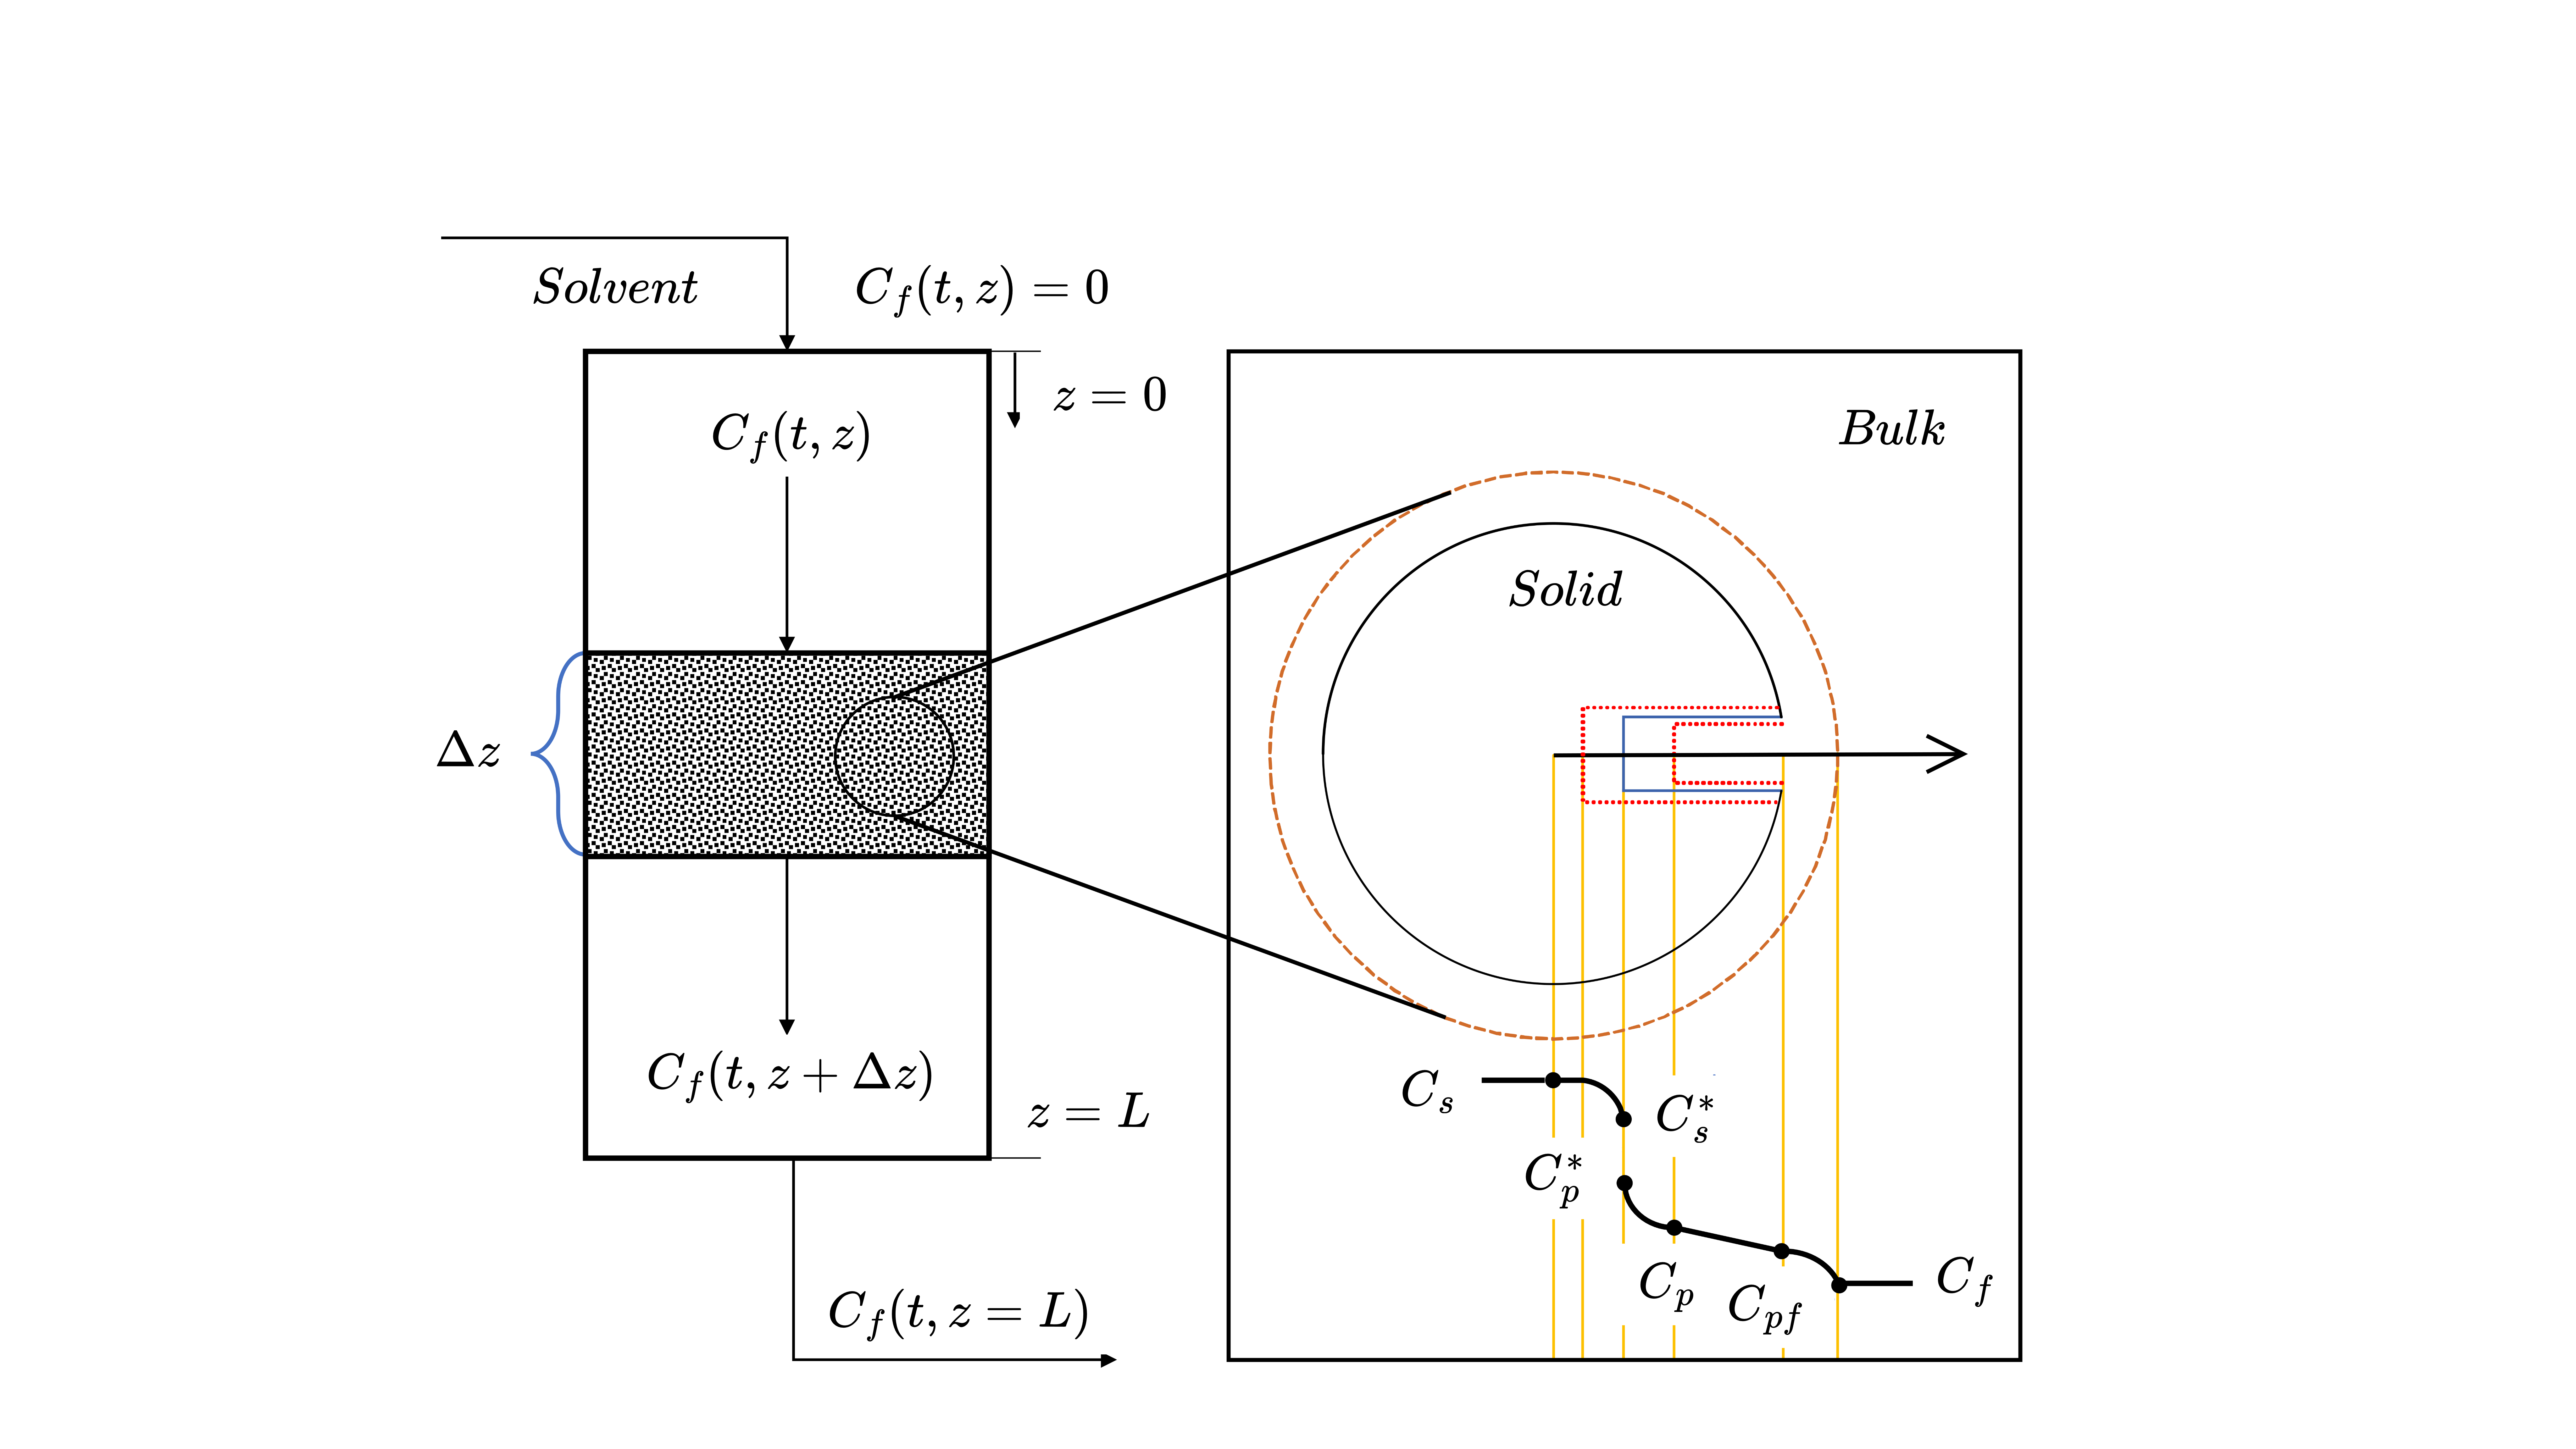
\includegraphics[trim = 45cm 0cm 60cm 20cm,clip,width=0.85\columnwidth]{Figures/SFE_PFD.drawio.png}	
			\caption{Mass transfer mechanism.}
			\label{fig: SFE_Mechanism}
		\end{figure}
		
		\citet{Bulley1984} suggest a process where the driving force for extraction is given by the difference between the concentration of the solute in the bulk, $c_f$, and in the centre of the pore, $c_p^*$. According to the equilibrium relationship, the concentration $c_p^*$ is in equilibrium with $c_s$. The rate of extraction is thus $r_e\left(c_f - c^*_p(c_s)\right)$. In contrast, \citet{Reverchon1996} proposes a driving force given by the difference between $c_s$ and $c_p^*$. As given by Equation \ref{Model_kinetic_basic}, the concentration $c_p^*$ is determined by the equilibrium relationship with $c_f$:
		
		{\footnotesize
			\begin{equation} \label{Model_kinetic_basic}
				r_e = \cfrac{D_i}{\mu l^2 }\left(c_s - c_p^* \right)
		\end{equation} }
		
		where $\mu$ is sphericity, $l$ a characteristic dimension of particles that can be defined as $l = r/3$, $r$ is the mean particle radius, $D_i$ corresponds to the overall diffusion coefficient and $c_P^*$ is the concentration at the solid-fluid interface (which according to the internal resistance model is supposed to be at equilibrium with the fluid phase). 
		
		According to \citet{Bulley1984}, a linear equilibrium relationship (Equation \ref{Linear_equilibirum}) can be used to find the equilibrium concentration of the solute in the fluid phase $c_f^*$ based on the concentration of the solute in the solid phase $c_s$:
		
		{\footnotesize
			\begin{align} \label{Linear_equilibirum}
				c_f^* &= k_p c_s
		\end{align} }
		
		The volumetric partition coefficient $k_p$ acts as an equilibrium constant between the solute concentration in one phase and the corresponding equilibrium concentration at the solid-fluid interphase. \citet{Spiro2007} proposed a definition of the mass partition coefficient $k_m$ and the solid density $\rho_s$ as 
		
		{\footnotesize
			\begin{align}
				k_m = \cfrac{k_p \rho_s}{\rho_f}
		\end{align} }
		
		According to \citet{Reverchon1996}, the kinetic term becomes
		
		{\footnotesize
			\begin{equation}
				\label{Model_kinetic_no_sat}
				r_e = \cfrac{D_i}{ \mu l^2 } \left(c_s - \cfrac{\rho_s c_f}{k_m \rho_f} \right)
		\end{equation} }
		
		%\subfile{Saturation}
		\subsubsection{Uneven solute distribution in the solid phase} \label{CH: Gamma_Function}
		
		Following the idea of the broken-and-intact cell (BIC) model (\citet{Sovova2017}), the internal diffusion coefficient $D_i$ is considered to be a product of the reference value of $D_i^R$ and the exponential decay function $\gamma$, as given by Equation \ref{EQ: C_sat_function}:
		
		{\footnotesize
			\begin{equation}
				D_i = D_i^R \gamma(c_s) = D_i^R \exp \left( - \Upsilon \left( 1-\cfrac{ c_s }{c_{s0}} \right) \right) \label{EQ: C_sat_function}
		\end{equation} }
		
		where  ${\color{black}\Upsilon}$ describes the curvature of the decay function. Equation \ref{Model_kinetic} describes the final form of the kinetic term:
		
		{\footnotesize
			\begin{equation}
				\label{Model_kinetic}
				r_e = \cfrac{D_i^R \gamma }{ \mu l^2 } \left( c_s  - \cfrac{\rho_s c_f }{ k_m \rho_f }  \right)
		\end{equation} }
		
		The $\gamma$ function limits the solute's availability in the solid phase. Similarly to the BIC model, the solute is assumed to be contained inside the cells, some of which are open because the cell walls have been broken by grinding, with the rest remaining intact. The diffusion of solute from a particle's core takes more time than the diffusion of solute close to the outer surface. The same idea can be represented by the decaying internal diffusion coefficient, where the decreasing term is a function of the solute concentration in the solid. 
		
		An alternative interpretation of the decay function $\gamma$ involves taking into account the porous structure of the solid particles, where the pores are initially saturated with the solute. During extraction, the solute within these pores gradually dissolves into the surrounding fluid. Initially, the solute molecules near the pore openings dissolve and diffuse rapidly due to the short diffusion paths. As extraction progresses, the dissolution front moves deeper into the pore structure and solute from the inner regions of the pores begins to dissolve. The diffusion of solute molecules from the interior of the pores to the external fluid becomes progressively slower because the effective diffusion path length increases. This lengthening of the diffusion path enhances mass transfer resistance, reducing the overall diffusion rate. 
		
		In an extreme case, this model could be compared with the shrinking core (SC) model presented by \citet{Goto1996}, where the particle radius is reduced as the solute content in the solid phase decreases. In the SC model, the reduction in particle size leads to significant changes in both the diffusion path length and the surface area available for mass transfer. The diminishing particle size increases the diffusion path within the remaining solid core and decreases the external surface area, both of which contribute to a slower extraction rate. When comparing this to the varying diffusion coefficient in our model, some conceptual similarities can be noticed.
		
		\subsubsection{Empirical correlations}
		
		The empirical correlations for $D_i$ and $\Upsilon$ were derived by \citet{Sliczniuk2024} and validated for temperatures of $30 - 40~^\circ C$, pressures of $100 - 200$ bar and mass flow rates of $3.33-6.67 \cdot 10^{-5}$ kg/s. Figures \ref{fig:Correlation_Di} and \ref{fig:Correlation_Gamma} show the results of multiple linear regression applied to parameter estimation solutions and selected independent variables. The region marked with the white dashed line represents the confidence region where the model has been tested. Both correlations should be equal or greater than zero to avoid unphysical behaviour such as reverse mass transfer. The multiple linear regression functions are combined with the rectifier function to ensure non-negativity.
		
		\begin{figure}[!ht]
			\centering
			
\includegraphics[trim = 0.0cm 0.0cm 0.0cm 0.0cm,clip,width=0.9\columnwidth]{/Di_1.png}
			\caption{Multiple linear regression $D_i^R = f(Re, F)$.}
			\label{fig:Correlation_Di}
		\end{figure}
		
		\begin{figure}[!ht]
			\centering
			
\includegraphics[trim = 0.0cm 0.0cm 0.0cm 0.0cm,clip,width=0.9\columnwidth]{/Gamma_1.png}
			\caption{Multiple linear regression $\Upsilon = f(Re, F)$.}
			\label{fig:Correlation_Gamma}
		\end{figure}
				
		\subsubsection{Heat balance} \label{CH: heat_balance}
		
		The heat balance equation describes the evolution of enthalpy in the system, given by Equation \ref{EQ:Enthalpy_equation}:
		
		{\footnotesize
			\begin{equation} \label{EQ:Enthalpy_equation}
				\cfrac{\partial \left(\rho_f {\color{black}h} A_f\right)}{\partial t} = - \cfrac{\partial \left( \rho_f {\color{black}h}  v \right)}{\partial z} + \cfrac{\partial \left(P A_f\right)}{\partial t} + \cfrac{\partial}{\partial z} \left( k \cfrac{\partial T}{\partial z} \right)
			\end{equation}
		}
		
		If the value of enthalpy $h$ is known from the time evolution of the energy equation and pressure $P$ is known from measurement, then the temperature $T$ can be reconstructed based on the departure function. The departure function is a mathematical function that characterises the deviation of a thermodynamic property (enthalpy, entropy or internal energy) of a real substance from that of an ideal gas at the same temperature and pressure. As presented by \citet{Gmehling2019}, the enthalpy departure function for the Peng-Robinson equation of state is defined by Equation \ref{EQ:Enthalpy_PR}:
		
		{\footnotesize
			\begin{equation}
				{\color{black}h}-{\color{black}h}^{id}={\color{black}R}T \left[{\color{black}T_r}({\color{black}Z}-1) -2.078(1+{\color{black}\kappa} ){\sqrt { {\color{black}\alpha}\left(T\right) } } \ln \left(\cfrac{{\color{black}Z}+\left( 1+\sqrt{2} \right){\color{black}B}}{{\color{black}Z}+\left( 1-\sqrt{2} \right){\color{black}B}}\right)\right]
				\label{EQ:Enthalpy_PR}
			\end{equation}				
		}
		
		where $\alpha$ is defined as $\left( 1+\kappa \left( 1 - \sqrt{T_r} \right) \right)^2$, $T_r$ is the reduced temperature, $P_r$ is the reduced pressure, $Z$ is the compressibility factor, $\kappa$ is a quadratic function of the acentric factor and $B$ is calculated as $0.07780\frac{P_r}{T_r}$.
		
		Equation \ref{EQ:Enthalpy_PR} requires a reference state, which is assumed to be $T_{ref}=298.15$ K and $P_{ref}=1.01325$ bar.
		
		A root finder can be used to find a temperature value that minimises the difference between the value of enthalpy coming from the heat balance and the departure functions. The root-finding procedure is repeated at every time step to find a temperature profile along the spatial direction $z$.
		
		{\footnotesize
			\begin{equation}
				\min_T \left( \underbrace{h\left(t,x\right)}_{\text{Heat balance}} - \underbrace{h\left(T,P,\rho_f\left(T,P\right)\right)}_{\text{Departure function}} \right)^2
				\label{EQ:Enthalpy_root}
			\end{equation}
		}
		
		\subsubsection{Pressure term} \label{CH: Pressure}
		
		As explained in Section \ref{CH:Governing_equations_chapter}, the pressure in the low-velocity region remains nearly constant due to the small pressure wave propagation occurring at the speed of sound. Under such conditions, the term $\partial P/\partial t$ can be approximated by a forward difference equation, describing the pressure change over a small time step $\Delta t$. The pressure $P$ in the system is treated as a state variable, while the incoming pressure at the new time step $P_{in}$ is treated as a control:
		
		{\footnotesize
			\begin{equation}
				\frac{\partial {\color{black}P}}{\partial t} \approx \frac{{\color{black}P_{in}} - {\color{black}P} }{\Delta t}
		\end{equation}}
		
		Such a simplified equation allows for instantaneous pressure. In a real system, the pressure dynamics would depend on the behaviour of the pump and the back-pressure regulator, which introduce additional inertia and resistance to pressure changes, leading to gradual pressure build-up.
		
		\subsubsection{Extraction yield} \label{CH: Yield}
		
		The process yield is calculated according to Equation \ref{Model_measurment_1}, as presented by \citet{Sovova1994a}. The measurement equation evaluates the solute's mass at the extraction unit outlet and sums it up. The integral form of the measurement (Equation \ref{Model_measurment_1}) can be transformed into the differential form (Equation \ref{Model_measurment_2}) and augmented with the process model.
		
		{\footnotesize
			\begin{align} 
				\label{Model_measurment_1}
				y &= \int_{t_0}^{t_f} \cfrac{F}{\rho_f} c_f \biggr\rvert_{z=L} dt \\
				\cfrac{dy}{dt} &= \qquad \cfrac{F}{\rho_f} c_f \biggr\rvert_{z=L} 
				\label{Model_measurment_2}
		\end{align}	}

		The measurement error can be obtained based on the accuracy of the measuring device, or empirically from the spread of data around the model output. The first approach can be utilised only in the absence of external error sources. Given the imperfections of the experimental setup, such as delayed measurements and residuals of the product in pipes and the draining vessel, it was decided that the second approach is more suitable for this work. Based on the \citet{Sliczniuk2024}, the empirical measurement error was estimated to be 0.03.
		
		\subsubsection{Initial and boundary conditions} 
		It is assumed that the solvent is free of solute at the beginning of the process $c_{f0}=0$, that all the solid particles have the same initial solute content $c_{s0}$ and that the system is isothermal, hence the initial state is $h_0$. The fluid at the inlet is considered not to contain any solute. The initial and boundary conditions are defined as follows:
		
		{\footnotesize
			\begin{align*}
				&c_f(t = 0, z) = 0  && c_s(t = 0, z) = c_{s0} && h(t = 0, z) = h_0 \\
				&c_f(t,   z=0) = 0  && h(t, z=0) = h_{in}  && \frac{\partial c_f(t,z=L)}{\partial x} = 0 \\
				&\frac{\partial h(t,z=L)}{\partial x} = 0   && c_s(t, z=\{0,L\}) = 0 && y(0) = 0 \quad P(0) = P_0 \\
		\end{align*} }
		
		\subsubsection{Discretisation methods}
		
		\begin{figure}[!h]
			\centering
			{\footnotesize
				\begin{align*}
					\dot{x} &= \cfrac{d x}{d t} = 
					\begin{bmatrix}
						\cfrac{d c_{f,1}}{d t} 	  \\
						\vdots					  \\
						\cfrac{d c_{f,N_z}}{d t} \\
						\\ \hline \\
						\cfrac{d c_{s,1}}{d t} 	  \\
						\vdots					  \\
						\cfrac{d c_{s,N_z}}{d t} \\
						\\ \hline \\
						\cfrac{d h_1}{d t} 	  \\
						\vdots 					  \\
						\cfrac{d h_{N_z}}{d t} \\
						\\ \hline \\
						\cfrac{d P}{d t} \\
						\\ \hline \\
						\cfrac{d y}{d t}
					\end{bmatrix}
					=
					\underbrace{\begin{bmatrix}
							G_1 \left( c_f,c_s,h; \Theta \right)\\ 
							\vdots\\ 
							G_{N_z} \left( c_f,c_s,h; \Theta \right)\\ 
							\\ \hline \\ \\
							G_{N_z+1} \left( c_f,c_s,h; \Theta \right)\\ 
							\vdots\\
							G_{2N_z} \left( c_f,c_s,h; \Theta \right)\\ 
							\\ \\ \hline \\ 
							G_{2N_z+1} \left( c_f,c_s,h; \Theta \right) \\
							\vdots\\
							G_{3N_z} \left( c_f,c_s,h; \Theta \right) \\ 
							\\ \\ \hline \\
							G_{3N_z+1} \left( c_f,c_s,h; \Theta \right) \\
							\\ \\ \hline \\
							G_{3N_z+2} \left( c_f,c_s,h; \Theta \right) 
					\end{bmatrix}}_{G \left( x; \Theta \right)} 
			\end{align*} }
			\caption{Discretised state space.}
			\label{fig:discretization}
		\end{figure}
		
		The method of lines is used to transform the process model equations into a set of ODEs denoted by $G(x;\Theta)$. For a derivative to be conservative, it must form a telescoping series. In other words, only the boundary terms should remain after adding all terms coming from the discretisation over a grid, and the artificial interior points should be cancelled out. Discretisation is applied to the conservative form of the model to ensure mass conservation. The backward finite difference is used to approximate the first-order derivative, while the central difference scheme approximates the second-order derivative $z$ direction. The length of the fixed bed is divided into $N_z$, i.e. equally distributed points in the $z$ direction. The state-space model after discretisation is denoted by $x$ and defined as shown in Figure \ref{fig:discretization}, where ${\color{black}x} \in \mathbb{R}^{N_x = 3N_z+2} $ and $\Theta \in \mathbb{R}^{N_\Theta =  N_{\theta} + N_u } $, $N_{\theta}$ is the number of parameters and $N_{u}$ is the number of control variables.
				
		\section{Variance-based sensitivity analysis} \label{chap:Sobol_Analysis}
		
		\citet{Sobol2001} suggested a framework that decomposes the variance of the model's or system's output into fractions that can be attributed to specific parameters. Variance-based measures of sensitivity are attractive because they assess sensitivity across the entire input space, handle nonlinear responses, and account for interactions terms. If the process model describes a dynamical system $G$, then it can be said that the model output is 
		
		{\footnotesize
			\begin{equation}
				Y\left(t|\theta\right) = G\left(x\left(t|\theta\right)\right) = G\left(x\left(t|\theta_1, \theta_2, \cdots, \theta_{n_\theta} \right)\right) 
		\end{equation} }
		
		where $Y$ is the model output, and $\theta$ is a parameter set. Sobol's suggested decomposing the function $G$ into summands of increasing dimensionality:
		
		{\footnotesize
			\begin{equation} \label{EQ:Sobol_decomposition_1}
				G\left(x\left(t|\theta_1, \theta_2, \cdots, \theta_{n_\theta} \right)\right) = G_0\left(t\right) + \sum_{i=1}^{n_\theta} G_i(t, \theta_i) + \sum_{i=1}^{n_\theta} \sum_{j=i+1}^{n_\theta} G_{ij} \left(t| \theta_i, \theta_j \right) + \cdots + G_{1...n_\theta}\left(t|\theta_1, \theta_2, \cdots, \theta_{n_\theta} \right)
		\end{equation} }
		
		If G is square-integrable and parameters are independent, the Sobol decomposition is unique. The constant term $G_0$ equals the expected value of the output, and all higher-order component functions have zero mean with respect to their respective arguments. The total unconditional variance is
		
		{\footnotesize
			\begin{equation}
				V(t) = \int_{\Omega} G^2\left(x\left(t|\theta\right)\right) d\theta - G_0^2(t)
		\end{equation}}
		
		where $\Omega$ denotes the $n_\theta$-dimensional unit hypercube to which the input. The partial variances, which form the components of the total variance decomposition, are obtained by integrating the squared summands of the ANOVA-HDMR decomposition:
		
		{\footnotesize
			\begin{equation} 
				V_{i_1, i_2, \cdots, i_s}(t) = \int_{0}^{1} \cdots \int_{0}^{1} 
				G^2_{i_1, \cdots, i_s} (t|\theta_{i_1}, \cdots, \theta_{i_s})\, 
				d\theta_{i_1} \cdots d\theta_{i_s}
		\end{equation}}
		
		where $1 \leq i_1 < \cdots < i_s \leq n_\theta$ and $s = 1, \ldots, n_\theta$. Since the model parameters are assumed to be statistically independent, and the summands in the decomposition are constructed to have zero mean and to be mutually orthogonal, the total variance decomposes into the sum of partial variances:
		
		{\footnotesize
			\begin{equation} \label{EQ:Sobol_decom}
				V(t) = \sum_{i=1}^{n_\theta}V_i(t) 
				+ \sum_{i=1}^{n_\theta-1}\sum_{j=i+1}^{n_\theta} V_{ij}(t) 
				+ \cdots + V_{1, \cdots, n_\theta}(t)
		\end{equation}}
		
		In this way, the variance contributions to the total output variance of individual parameters and parameter interactions can be determined. These contributions are characterised by the ratio of the partial variance to the total variance, the Sobol's sensitivity indices. The first-order Sobol' index, $S_i(t) = \frac{V_i(t)}{V(t)}$, is a measure for the variance contribution of the individual parameter $\theta_i$ to the total model variance. The partial variance $V_i(t)$ is given by the variance of the conditional expectation $V_i(t) = V[\mathbb{E}(Y(t|\theta_i))]$ and is called the "main effect" of $\theta_i$ on $Y(t)$. It can be described as the fraction of the model output variance that would disappear on average when $\theta_i$ is fixed to a value in its range. The impact on the model output variance of the interaction between $\theta_i$ and $\theta_j$ is given by the second order Sobol' index, $S_{ij} = \frac{V_{ij}}{V}$, and the total Sobol' index $S_{Ti} = S_i + \sum_{j \neq i} S_{ij} + \sum_{j \neq i} \sum_{k \neq i, k>j} S_{ijk} $.
		
		In additive models with independent input factors, $S_{Ti}$ and $S_i$ are equal for each parameter, and the sum of all first-order Sobol’ indices equals 1. In contrast, non-additive models may exhibit interaction effects, resulting in $S_{Ti} \geq S_i$, with strict inequality for parameters involved in interactions. When interactions contribute to output variance, the sum of the first-order indices is less than 1. Conversely, the sum of the total-effect indices exceeds 1 in the presence of interaction effects, as interaction contributions are included in the total-effect index of each participating parameter. Therefore, the difference between $S_{Ti}$ and $S_i$ quantifies the extent to which parameter $\theta_i$ participates in interactions with other parameters.
		
		To compute the variance and obtain sensitivity measures, Sobol proposed a shortcut calculation based on the assumption that the decomposition's summands are mutually orthogonal. The shortcut is attained by transforming the double-loop integral into an integral of the product of $G(\theta_{j1}, \cdots, \theta_{k-s'}, \theta_{1}, \cdots, \theta_{s})$ and $G(\theta'_{j1}, \cdots, \theta'_{k-s'}, \theta_{1}, \cdots, \theta_{s})$.
		
		Due to the complexity and nonlinearity of process models, analytical solutions are difficult to obtain; consequently, Monte Carlo integration is often used. The estimation of the total unconditional variance becomes:
		
		{\footnotesize
			\begin{align}
				V(t) \approx \hat{V}(Y(t)) &= \frac{1}{n-1} \sum_{m=1}^{n} G^2(\theta_m) - \hat{G}_0^2 \\
				\hat{G}_0 &\approx \frac{1}{n} \sum_{m=1}^{n} G(t|\theta_m)
		\end{align}}
		
		Here, $\hat{G}$ denotes the estimate, $\theta_m$ refers to a sampled set of input parameters, and $n$ indicates the number of samples. According to \citet{Saltelli2010}, two independent input sample matrices of size $n \times n_\theta$ (the "sample" matrix $M_1$ and the "resample" matrix $M_2$) are used to compute the Monte Carlo integrals, where $n$ is the sample size and $n_\theta$ is the number of parameters. Each row in $M_1$ and $M_2$ corresponds to a possible parameter combination for the model. The parameter ranges in these matrices are scaled between 0 and 1. These two matrices are required to construct the sample sets for $G(\theta_{j1}, \cdots, \theta_{k-s'}, \theta_{1}, \cdots, \theta_{s})$ and $G(\theta'_{j1}, \cdots, \theta'_{k-s'}, \theta_{1}, \cdots, \theta_{s})$.
		
		After generating the two primary matrices, the Saltelli algorithm constructs additional input matrices by substituting columns from the base matrix with the corresponding columns from the resample matrix. This substitution isolates the influence of each parameter when computing sensitivity indices. The total number of matrices equals the number of parameters plus two, reducing computational complexity.
		
		\subsection{Analysis of the first-order indices}
		
		The GSA is applied to quantify how operating conditions (temperature between 30 and 40 $^\circ$C, pressure between 100 and 200 bar, and mass flow rate between $3.3$ and $6.7\times 10^{-5}$ kg/s) influence the extraction yield over time. The analysis was carried out with a sample size of $N = 10^5$ on a one-minute time grid. The resulting trajectories are shown in Figure \ref{fig:Yield_CI}.
		
		\begin{figure}[h!]
			\centering
			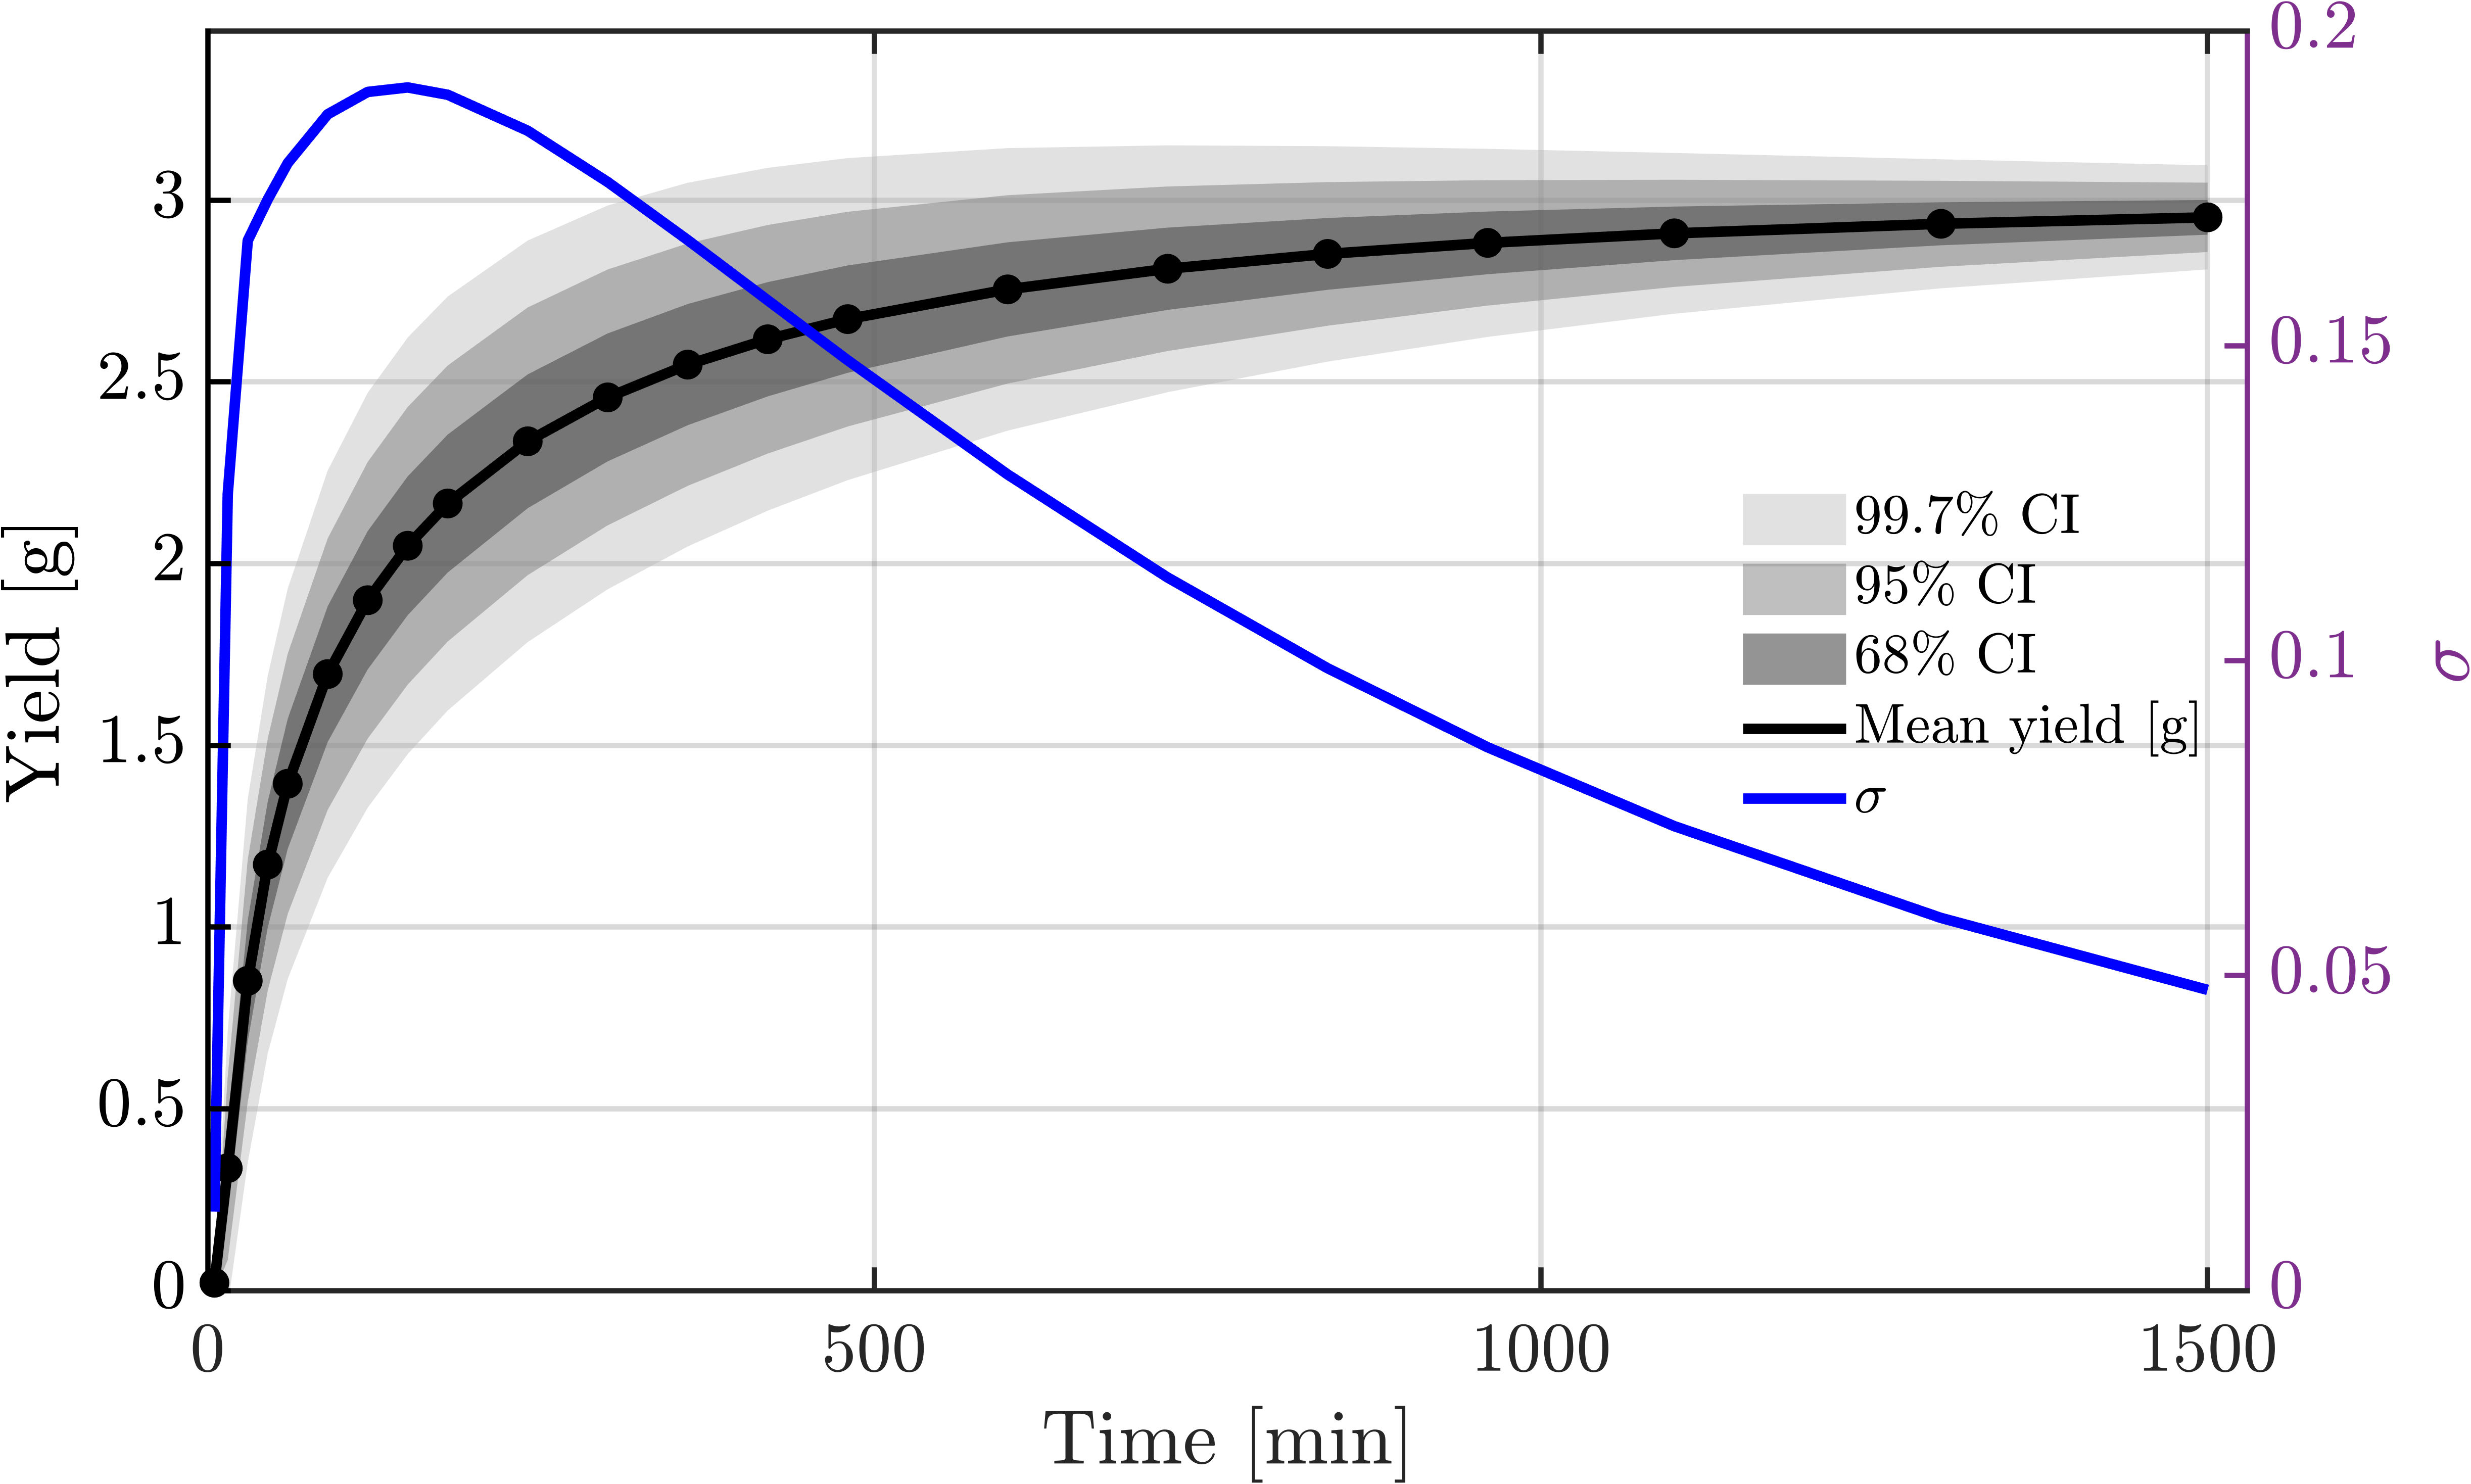
\includegraphics[trim = 0.0cm 0.0cm 0.0cm 0.0cm,clip,width=\columnwidth]{Figures/Results/CI.png}
			\caption{Predicted yield curve and bootstrap confidence interval}
			\label{fig:Yield_CI}
		\end{figure}
		
		Figure \ref{fig:Sobol} presents the temporal evolution of the first-order and total Sobol indices. Three distinct regimes are identified.
		
		\emph{Convection-limited regime}: During this regime, mass flow rate predominantly determines output variance. The value of $S_F$ increases from $0.85$ at $t = 5$ min to a maximum of $0.98$ at $t = 30$ min, while $S_P$ and $S_T$ decrease toward zero ($S_P = 0.003$ and $S_T = 10^{-4}$ at $t = 30$ min). In this period, the fluid-phase remains far from saturation, allowing the solvent to remove solute as rapidly as it is supplied. Thermodynamic properties exert only a minor influence on yield in this regime. The small, nonzero $S_P$ observed at the earliest time point ($S_P = 0.10$ at $t = 5$ min) indicates density-driven differences in the propagation of the concentration front.
		
		\emph{Transitional regime}: As the accessible solute becomes depleted, the bed gradually transitions toward a solubility-limited side, and the importance of pressure grows monotonically. $S_F$ decreases from $0.93$ at $t = 60$ min to $0.49$ at $t = 1100$ min, while $S_P$ increases from $0.04$ to $0.46$ over the same interval. Temperature contributes a small but progressively larger share ($S_T$ rises from $0.004$ to $0.06$). Low values of $S_T$ can be explained by the narrow temperature operating range.
		
		\emph{Equilibrium-influenced regime}: In this regime, pressure emerges as the largest single contributor, with $S_P = 0.49$, $S_F = 0.41$, and $S_T = 0.09$ at $t = 1500$ min. Notably, $S_P$ and $S_F$ remain of similar magnitude. Throughout the 1500 min window, the process does not become strongly thermodynamic-dominated, in contrast to the early dominance of flow. 
		
		\begin{figure}[h!]
			\centering
			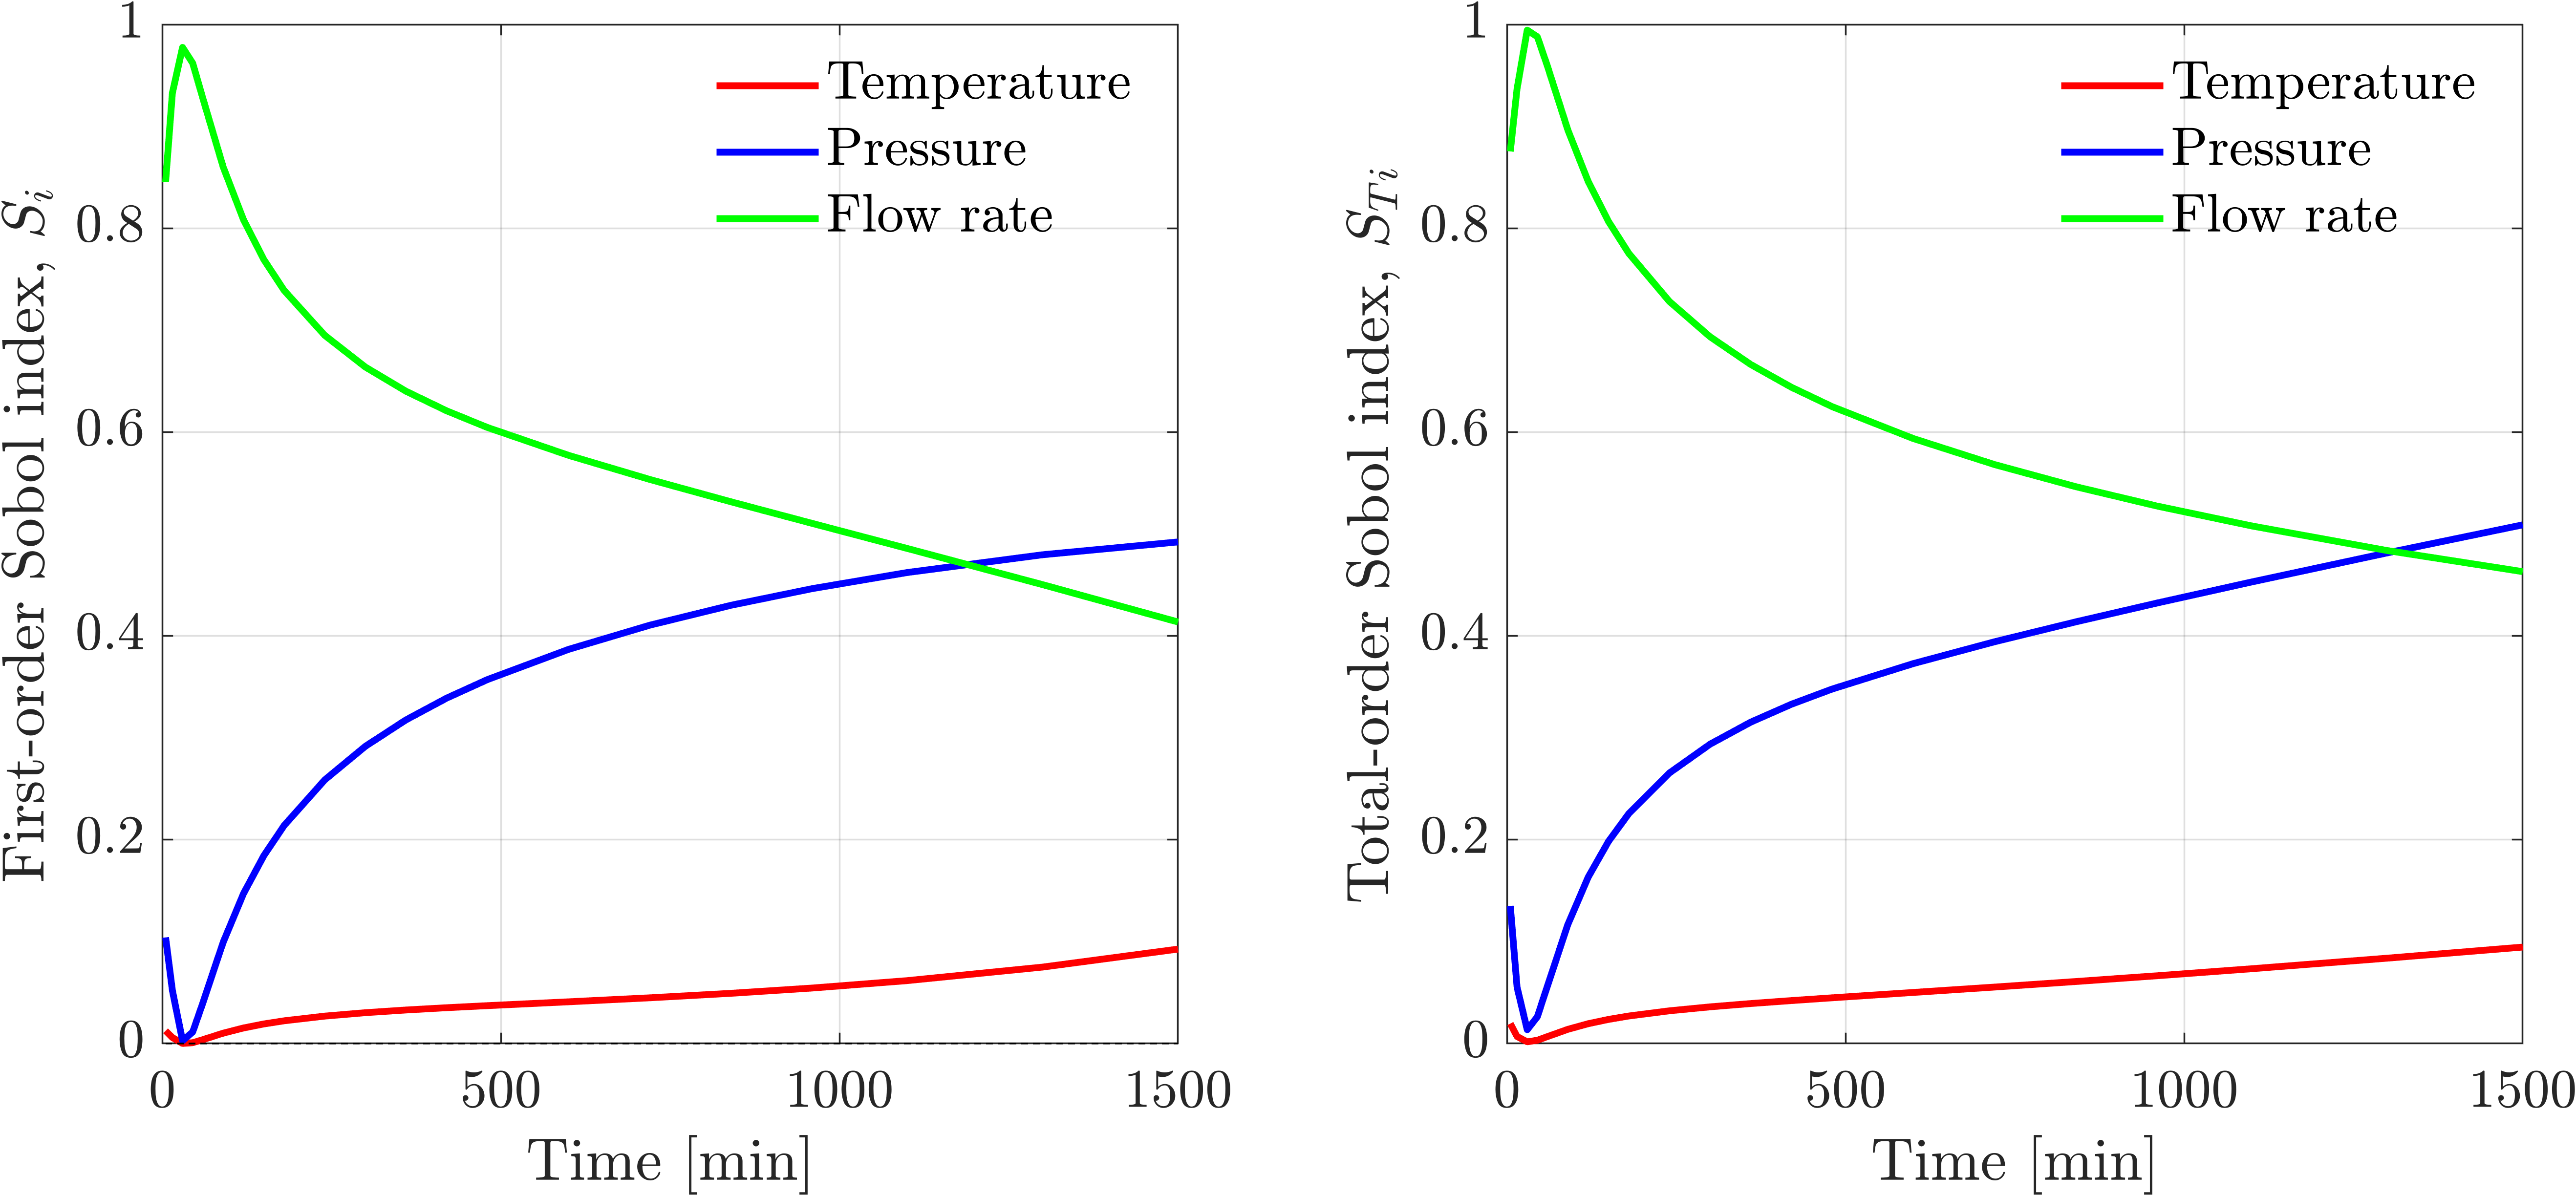
\includegraphics[trim = 0.0cm 0.0cm 0.0cm 0.0cm,clip,width=\columnwidth]{Figures/Results/Sobol.png}
			\caption{Time evolution of the first-order and total Sobol indices for temperature, pressure, and mass flow rate.}
			\label{fig:Sobol}
		\end{figure}
		
		Throughout the batch, the total indices ($S^T_i$) closely follow the first-order indices ($S_i$), and the sum $S_T + S_P + S_F$ remains within the range $[0.96, 1.01]$. Thus, the variance of the cumulative yield is explained almost entirely by additive first-order effects, with limited contribution from interactions.
		
		The evolution of the mean and standard deviation of the yield provides essential context for interpreting the Sobol estimates. The mean yield increases monotonically from $0.021$ to approximately $2.95$, indicating that the process approaches a plateau. In contrast, the standard deviation across the operating window reaches a maximum of approximately $0.19$ before decreasing steadily to $0.048$. As a result, the coefficient of variation decreases from about $0.59$ to approximately $0.016$. Consequently, late-time Sobol estimates are derived from a much smaller relative output variance. This observation explains why higher-order terms and closure diagnostics become more sensitive to estimator noise near the end of the batch, even though the first-order and total-order indices remain stable.
		
		\subsection{Analysis of the interaction terms}
		Second-order Sobol indices quantify the variance attributable to the joint variation of input pairs, beyond their individual effects. The third-order index completes the variance decomposition for three parameters. Throughout the batch, the total interaction budget remains within the range $0$–$0.04$. The individual second- and third-order indices are presented in
		Figure \ref{fig:Sobol_Interaction}.
		
		\begin{figure}[h!]
			\centering
			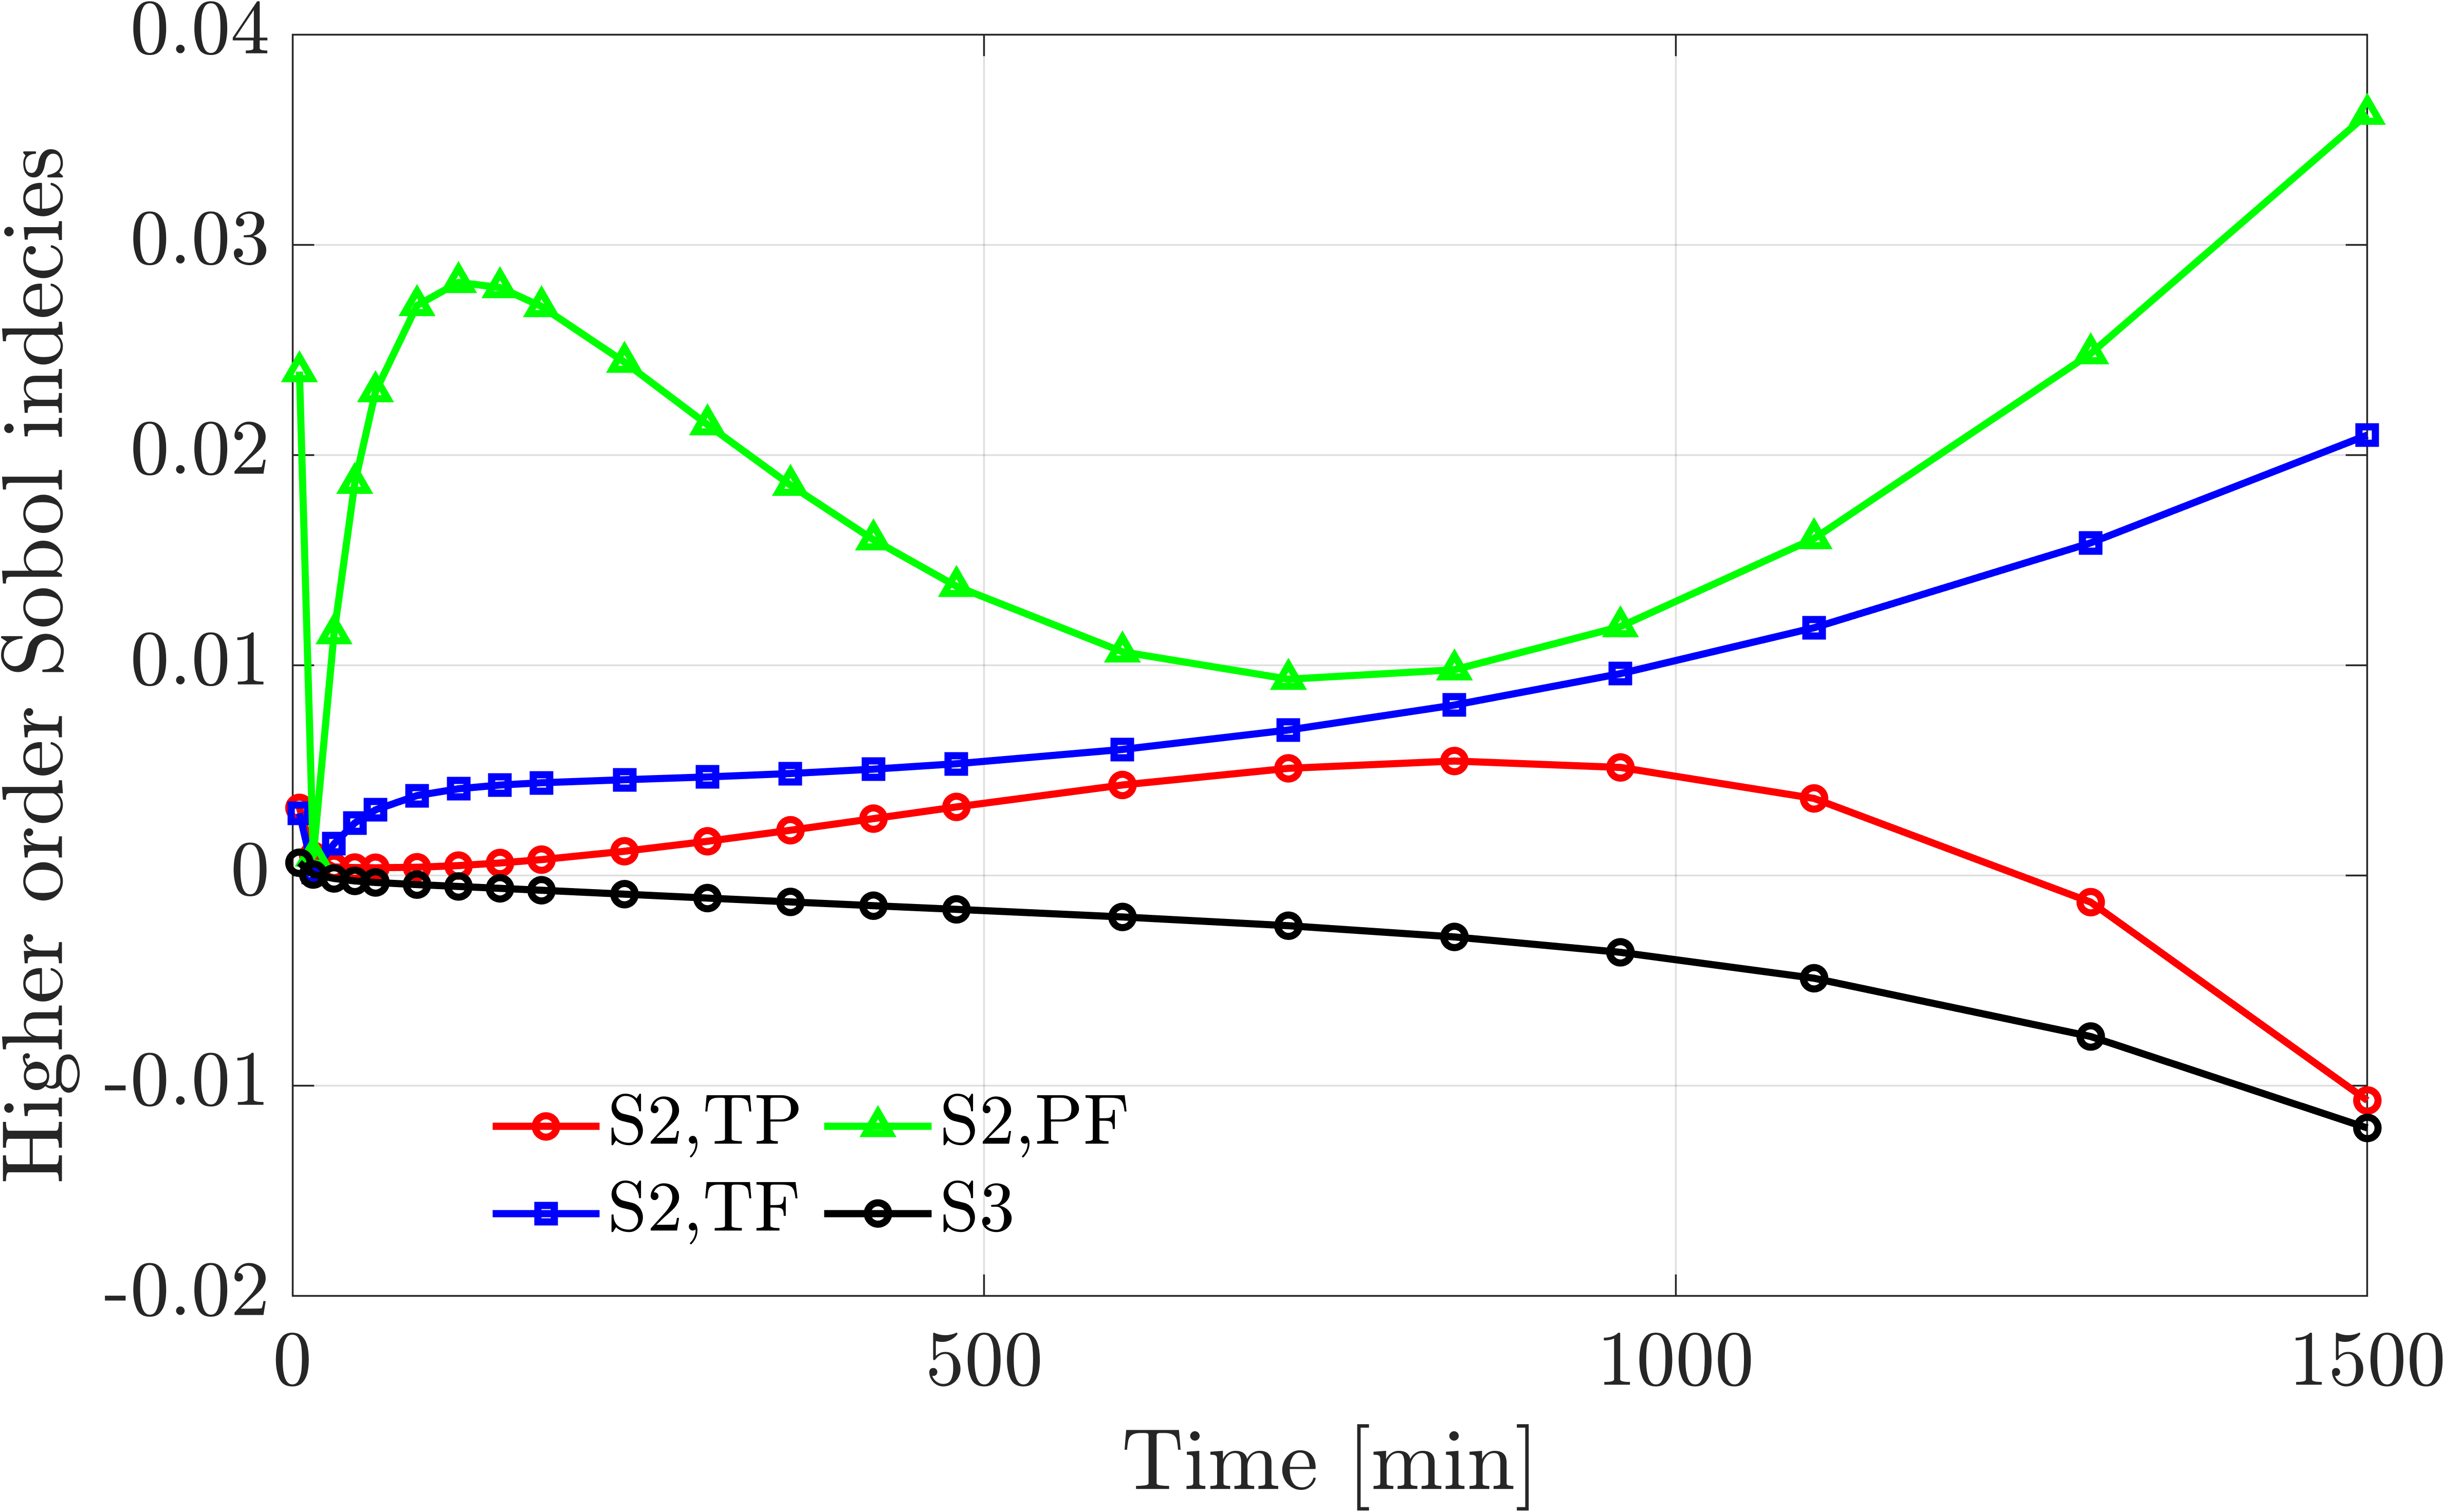
\includegraphics[trim = 0.0cm 0.0cm 0.0cm 0.0cm,clip,width=\columnwidth]{Figures/Results/High_Order_Interaction_effects.png}
			\caption{Time evolution of the second- and third-order Sobol interaction indices.}
			\label{fig:Sobol_Interaction}
		\end{figure}
		
		Among the pairwise terms, the pressure–flow interaction $S_{2,PF}$ exhibits the largest magnitude across most of the batch. This interaction increases sharply in the convection-limited regime, peaking at approximately $0.028$ near $t = 120$ min. It subsequently decreases during the transitional regime as the single-input effect of pressure accounts for a larger share of the variance, and then increases again in the late stage to $S_{2,PF} = 0.036$ at $t = 1500$ min. This non-monotonic profile aligns with the dependence of both the Re number, which is relevant in convection, and the solvent density and solubility, which are relevant near thermodynamic equilibrium.
		
		The $S_{2,TF}$ term remains small but increases monotonically from $0.003$ to $0.021$. This trend reflects the gradual increase in the importance of temperature-driven changes in $\rho$, $\mu$, and solubility over time.
		
		The temperature–pressure interaction $S_{2,TP}$ remains small throughout the batch. It increases only marginally at intermediate times, reaching values on the order of $0.005$, and becomes slightly negative at the latest times. Because Sobol variance components are non-negative by definition, these negative estimates are not considered meaningful. As the extraction yield approaches its plateau, the remaining variance within the operating window decreases, making weak interaction terms difficult to resolve accurately. Higher-order indices are interpreted qualitatively, while conclusions are drawn primarily from first-order and total-order trends.
		
		The independently estimated third-order index $S_3$ remains close to zero throughout the batch, with small negative values observed at later times ($ S_3 =- 0.012$). These values are attributed to estimator uncertainty rather than to physically meaningful negative variance contributions. The closure of the independently estimated decomposition, $\sum_i S_i + S_{2,TP}+S_{2,TF}+S_{2,PF}+S_3$,remains within approximately $4\%$ of unity, reaching a maximum value of about $1.04$. This result demonstrates acceptable consistency for interpreting the dominant sensitivity structure. Consequently, the third-order contribution is not significant from a practical perspective.
		
		% ===================================================
		% Section: Summary
		% ===================================================		
		
		\section{Conclusion} \label{CH: Conclusion}
		This work focus on application and comparison of variance-based diagnostic to measures an impact of controls on a SFE model. The analysis of results helped to identify which of controls is the most influential. Later the analysis was extended to investigate how a combination of controls affect the system. Due to dynamic nature of the model, a temporal evolution of the Sobol indices was observed. The results were analysed not only with respect to the future application of the dynamic optimization but also from the perspective of mass transfer theory.
		
		The model-based experimental design and control should consider the $P$–$F$ interaction throughout the batch, as well as the late-stage $T$–$P$ compensation. Treating the inputs as fully additive would overstate the variance attributable to pressure alone near the end of extraction. Second, the time evolution of the indices—from $S_F$ dominance, through a broad transition, to a regime where $S_P$ and $S_F$ are comparable—suggests that time-varying operating conditions could leverage different sensitivity structures at various process stages of the batch. This observation motivates extending the classical SFE into the dynamic operations.

% ===================================================
% Bibliography
% ===================================================
%% Loading bibliography style file
%\clearpage
%\newpage
%\bibliographystyle{model1-num-names}
\bibliographystyle{unsrtnat}
\bibliography{mybibfile}

%\clearpage \appendix \label{appendix}
%\section{Appendix} 
%\subfile{Sections/Qubic_EOS} \label{CH: EOS}
%\subsection{Cardano's Formula} \label{CH: Cardano}
%\subfile{Sections/Cardano}

%\clearpage
%\newpage

\nomenclature[A]{\(A\)}{Information matrix \nomunit{[-]}}
\nomenclature[A]{\(A\)}{Total cross-section of the bed \nomunit{$m^2$}}
\nomenclature[A]{\(A_f\)}{Cross-section of the bed occupied by the fluid \nomunit{$m^2$}}
\nomenclature[A]{\(B\)}{Pressure dependent parameter of P-R EoS \nomunit{$m^2$}}
\nomenclature[A]{\(B\)}{Weighted score vector \nomunit{[-]}}
\nomenclature[A]{\(C\)}{Weighted sum of squared deviations \nomunit{[-]}}
\nomenclature[A]{\(c_f\)}{Concentration of solute in the fluid phase \nomunit{kg/$m^3$}}
\nomenclature[A]{\(c_f^*\)}{Concentration of solute at the solid-fluid interface \nomunit{kg/$m^3$}}
\nomenclature[A]{\(c_{f0}\)}{Initial concentration of solute in the fluid phase \nomunit{kg/$m^3$}}
\nomenclature[A]{\(c_p\)}{Concentration of solute in the core of a pore \nomunit{kg/$m^3$}}
\nomenclature[A]{\(c_{pf}\)}{Concentration of solute at the pore opening \nomunit{kg/$m^3$}}
\nomenclature[A]{\(c_s\)}{Concentration of solute in the solid phase \nomunit{kg/$m^3$}}
\nomenclature[A]{\(c_s^*\)}{Concentration of solute at the solid-fluid interface \nomunit{kg/$m^3$}}
\nomenclature[A]{\(c_{s0}\)}{Initial concentration of solute in the solid phase \nomunit{kg/$m^3$}}
\nomenclature[A]{\(D_e^M\)}{Axial diffusion coefficient \nomunit{$m^2$/s}}
\nomenclature[A]{\(D_i\)}{Internal diffusion coefficient \nomunit{$m^2$/s}}
\nomenclature[A]{\(D_i^R\)}{Reference value of internal diffusion coefficient \nomunit{$m^2$/s}}
\nomenclature[A]{\(e\)}{Internal energy \nomunit{J/kg}}
\nomenclature[A]{\(F\)}{Mass flow rate \nomunit{kg/s}}
\nomenclature[A]{\(G\)}{Vector of discretized differential equations \nomunit{[-]}}
\nomenclature[A]{\(h\)}{Enthalpy \nomunit{kJ/kg}}
\nomenclature[A]{\(J\)}{Jacobian \nomunit{[-]}}
\nomenclature[A]{\(j\)}{Objective function \nomunit{[-]}}
\nomenclature[A]{\(k_m\)}{Mass partition coefficient \nomunit{[-]}}
\nomenclature[A]{\(k_p\)}{Volumetric partition coefficient \nomunit{[-]}}
\nomenclature[A]{\(L\)}{Length of the fixed bed \nomunit{m}}
\nomenclature[A]{\(l\)}{Characteristic dimension of particles \nomunit{m}}
\nomenclature[A]{\(n_\theta\)}{Number of analyzed parameters \nomunit{[-]}}
\nomenclature[A]{\(n_y\)}{Number of measurements \nomunit{[-]}}
\nomenclature[A]{\(N_z\)}{Number of discretized points in z-direction \nomunit{[-]}}
\nomenclature[A]{\(P\)}{Pressure \nomunit{bar}}
\nomenclature[A]{\(P_r\)}{Reduced pressure \nomunit{[-]}}
\nomenclature[A]{\(p\)}{Probability distribution model \nomunit{[-]}}
\nomenclature[A]{\(Q\)}{Weighting matrix \nomunit{[-]}}
\nomenclature[A]{\(Re\)}{Reynolds number \nomunit{[-]}}
\nomenclature[A]{\(r\)}{Particle radius \nomunit{m}}
\nomenclature[A]{\(r_e\)}{Mass transfer kinetic term \nomunit{kg/$m^3$/s}}
\nomenclature[A]{\(T\)}{Temperature \nomunit{K}}
\nomenclature[A]{\(T_{in}\)}{Inlet temperature \nomunit{K}}
\nomenclature[A]{\(T_{out}\)}{Outlet temperature \nomunit{K}}
\nomenclature[A]{\(T_r\)}{Reduced temperature \nomunit{[-]}}
\nomenclature[A]{\(t\)}{Time \nomunit{s}}
\nomenclature[A]{\(t_0\)}{Initial extraction time \nomunit{s}}
\nomenclature[A]{\(t_f\)}{Total extraction time \nomunit{s}}
\nomenclature[A]{\(u\)}{Superficial velocity \nomunit{m/s}}
\nomenclature[A]{\(v\)}{Linear velocity \nomunit{m/s}}
\nomenclature[A]{\(x\)}{State vector \nomunit{[-]}}
\nomenclature[A]{\(Y\)}{Yield measurement \nomunit{g}}
\nomenclature[A]{\(y\)}{Predicted extraction yield \nomunit{g}}
\nomenclature[A]{\(Z\)}{Compressibility factor \nomunit{[-]}}
\nomenclature[A]{\(z\)}{Spatial direction \nomunit{m}}

% Non-latin symbols
\nomenclature[B]{\(\mathcal{F}\)}{Fisher information \nomunit{[-]}}
\nomenclature[B]{\(\mathcal{R}\)}{Control cost matrix \nomunit{[-]}}

% Greek symbols
\nomenclature[C]{\(\alpha\)}{Temperature-dependent function in the P-R EoS \nomunit{[-]}}
\nomenclature[C]{\(\Delta_\theta\)}{Residual term of the parameters \nomunit{g}}
\nomenclature[C]{\(\Delta_y\)}{Residual term of the measurement error \nomunit{g}}
\nomenclature[C]{\(\epsilon\)}{Unobservable error \nomunit{g}}
\nomenclature[C]{\(\gamma\)}{Decaying function \nomunit{[-]}}
\nomenclature[C]{\(\kappa\)}{Quadratic function of the acentric factor \nomunit{[-]}}
\nomenclature[C]{\(\mu\)}{Sphericity coefficient \nomunit{[-]}}
\nomenclature[C]{\(\phi\)}{Bed porosity \nomunit{[-]}}
\nomenclature[C]{\(\pi\)}{Probability density \nomunit{[-]}}
\nomenclature[C]{\(\rho_f\)}{Fluid density \nomunit{kg/$m^3$}}
\nomenclature[C]{\(\rho_s\)}{Bulk density of solid \nomunit{kg/$m^3$}}
\nomenclature[C]{\(\Sigma\)}{Covariance matrix \nomunit{[-]}}
\nomenclature[C]{\(\Sigma_\theta\)}{Parameter uncertainty matrix \nomunit{[-]}}
\nomenclature[C]{\(\Sigma_Y\)}{Measurement covariance matrix \nomunit{[-]}}
\nomenclature[C]{\(\sigma\)}{Standard deviation \nomunit{[-]}}
\nomenclature[C]{\(\Theta\)}{Parameter space \nomunit{[-]}}
\nomenclature[C]{\(\theta\)}{Vector of analysed parameters \nomunit{[-]}}
\nomenclature[C]{\(\Upsilon\)}{Decay coefficient \nomunit{[-]}}
\nomenclature[C]{\(\varkappa\)}{An arbitrary function of \(\mathcal{A}\)}
\nomenclature[C]{\(\Xi\)}{Matrix of experimental conditions \nomunit{[-]}}
\nomenclature[C]{\(\xi\)}{Vector of experimental conditions \nomunit{[-]}}

% Abbreviations
\nomenclature[D]{BIC}{Broke-and-Intact Cell model}
\nomenclature[D]{DoE}{Design of Experiment}
\nomenclature[D]{HBD}{Hot Ball Diffusion}
\nomenclature[D]{m-DoE}{Model-based Design of Experiment}
\nomenclature[D]{P-R EoS}{Peng-Robinson Equation of State}
\nomenclature[D]{SC}{Shrinking Core}
\nomenclature[D]{SFE}{Supercritical Fluid Extraction}
\printnomenclature

\end{document}























